
\documentclass[oneside]{ausarbeitung}
\bibliography{latexlit}


% ----------------------------------------------------------------------

\begin{document}

%--- Sprachauswahl
% Erlaubte Werte:
%   \selectlanguage{english}
%   \selectlanguage{ngerman}
\selectlanguage{english}

%--- Art der Arbeit
% Erlaubte Werte:
%   \Praxissemesterbericht
\Projektbericht
%   \Bachelorarbeit
%   \Seminararbeit
%   \Masterarbeit

%--- Studiengang:
% Erlaubte Werte:
%   \Informatik
%   \Elektronik
%   \DataScience
\Informatik

\title{Epidemics}

\author{Sascha Mößle, Tim Staudenmaier}
\matrikelnr{75987, 75981}

%--- Ist der Erstbetreuer (\examinerA) an der Hochschule ein Professor?
% Erlaubte Werte:
%   \examinerIsAProfessortrue   % Ja
%   \examinerIsAProfessorfalse  % Nein
\examinerIsAProfessortrue   % Ja

%--- Betreuer
\examinerA{Prof.~Dr.~Thomas~Thierauf}
%\examinerB{Prof.~Dr.~Ulrich~Klauck}

%--- Einreichungsdatum
\date{14.3.2023}

%--- Angaben zur Firma
% Auskommentieren, wenn die Arbeit nicht bei einer ext. Firma gemacht wurde.
%\companyname{Beispielfirma}
%\industrialsector{Beispielbranche}
%\department{Beispielabteilung}
%\companystreet{Beispielstr. 1}
%\companycity{12345 Musterstadt}

%--- Angaben zum Betreuer bei dieser Firma
%\advisorname{Name des Betreuers}
%\advisorphone{(01234) 567-890}
%\advisoremail{name@company.xxx}

%--- Titelseite Anzeigen
\maketitle
\cleardoublepage

%---
\pagenumbering{roman}
\setcounter{page}{1}

%--- Firmendaten Anzeigen
% Auskommentieren, wenn die Arbeit nicht bei einer ext. Firma gemacht wurde.
%\makeworkplace
%\cleardoublepage

%--- Eidesstattliche Erklärung anzeigen
\makeaffirmation
\cleardoublepage

%---
\begin{abstract}
 Epidemic diseases are an important area of studies. During the history of humans there
 were multiple instances of epidemics singificantly affecting large parts of the world.
 One recent example would be the Corona virus which brought most parts of the world to a 
 standstill. The area of epidemics focuses on such contagious diseases which spread from
 person to person, like Corona of influenza.

 Depending on the characteristics of the virus epidemics can have a very different progression.
 Some may explosively affect the whole world while not causing many casualties while others
 spread very slowly but linger for a long time with a high fatality rate. An important 
 part of studying these diseases is simulating how different diseases could affect the world.
 The simulation of such diseases can be accomplished using network graphs. This paper introduces
 a model wich can be used for simulation and explains how the program that allows to simulate
 a disease using that model is built.
\end{abstract}
%-----------------------------------------------------------------------
\cleardoublepage
\tableofcontents

%---
\listoffigures

%---


\cleardoublepage
\pagenumbering{arabic}
\setcounter{page}{1}

\algrenewcommand\algorithmicrequire{\textbf{Input:}}
\algrenewcommand\algorithmicensure{\textbf{Output:}}

% ----------------------------------------------------------------------

\chapter{Introduction}
\label{cha:introduction}
\section{Motivation}
An epidemic outbreak can have a major impact on the world. Past epidemics have shown that
if we do not know how to counteract an epidemic outbreak and are not prepared for 
such cases, a new disease can cause the death of major parts of the world. The black
death caused the death of about 30\% to 60\% of all Europeans (75-200 million)
during the 1300s \cite{blackDeath}.
To better understand such scenarios simulations play an important role since studying real
cases of epidemic outbreaks is difficult as there are only so many in the history of humans.
Also it is important in case an outbreak happens to be able to simulate the next few days/weeks
to accurately predict how the epidemic will evolve.

For this reason this work will discuss an approach to simulate such epidemics by modeling
networks of persons and then simulating the spreading of diseases with different properties
in these networks.

\section{Problem definition}
A model of the social network the disease is spreading in is curcial to the simulation.
Depending on the transmission method of the disease this network can be highly connected in 
the case of a disease with airborne transmission or have only few connections for diseases
that are for example sexually transmitted. In addition to that different diseases can spread
completely different in the same social network even if the have the same transmission method
because the characteristics of the disease also play an important role in how it spreads. 
As suggested by Easley and Kleinberg \cite{networks}
the transmission of computer viruses works in a similar way an thus is also able to be modeled
by using networks.

The networks that can be created using the app must be able to model different social
networks. The important part for the epidemics simulation is the modeling of the amount
of contacts with other humans each human has. Since each group can contain a significant amount
of members an efficient method for creation networks with large amounts of nodes is required, which
still allows to model most social networks.

A method to visually display these networks in a clear way is required. The visual 
representation must still be usable with large amounts of nodes (eg. over 100,000 nodes).
To make the visualization of the network more usable some settings need to be provided
to alter the displayed network, like hiding certain connections or nodes. It also needs
ways to represent the current state of the network in respect to the spread of the diseases.

The app also needs to allow for creation of multiple diseases with different properties.
To simulate various epidemic scenarios properties like the infectiousness, duration of illnes
or fatality need to be editable. 

The app should be able to simulate multiple diseases at the same time. The simulation needs
to take into account which humans have contact with each other and then simulate the spreading
of the diseases according to the properties of each disease and group of humans.

During the simulation the app will collect statistics to allow a review of key information
after a simulation, like the amount of new infections over time.

\chapter{Theory of modeling epidemics}
\label{cha:general_principles}
The models the app developed in this work uses are based on chapters 19-21 of the book
"Networks Crowds and Markets" Easley and Kleinberg \cite{networks}.

\section{Simplest model}
The first model proposed by Easley and Kleinberg \cite{networks} uses a very simplistic
representation of networks. The network is represented as a tree with each layer representing
the nodes who come into contact with infected nodes form the previous cycle. The root
of the tree is the first person to contract the disease in the social network. During the
first cycle the $k$ nodes at a depth of 1 may or may not get infected with the disease based
on the infectiousness of the disease. During the second cycle each of these $k$ nodes
now comes into contact with $k$ other nodes at a depth of 2. This means during the second
cycle $k \cdot k = k^2$ people are potentially at risk of infection. During each cycle the
amount of people that come into contact with the disease increases by a factor of $k$ for
a total of $k^{cycle}$ that potentially come into contact with the disease during each cycle.
Figure \ref{fig:tree_network} shows a possible network structure.

\begin{figure}
    \centering
    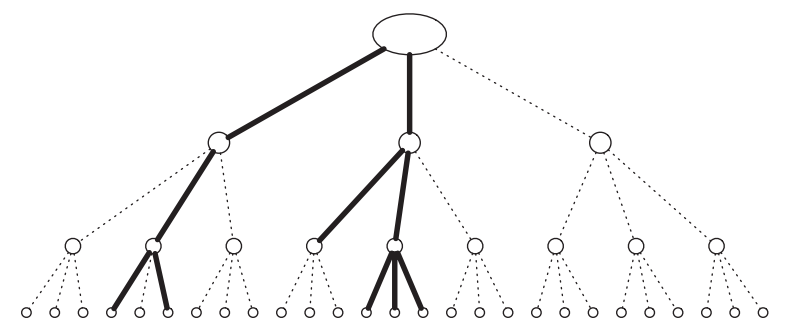
\includegraphics[width=0.5\linewidth]{images/network_tree.png}
    \caption{Tree representation of a network showing the spread of a disease (source: \cite{networks})}
    \label{fig:tree_network}
\end{figure}

The book \cite{networks} also explains the concept of the reproductive number $R_0$ in
relation to this network. $R_0$ is the expected number of new cases of the disease
caused by a single infected individual. In the case of the tree network this means 
$R_0 = pk$ with $p$ being the infectiousness of the disease. If $R_0 > 1$ the amount
of cases will increase over time because each person infects more than one other person
on average. Thus there is a possibility that the disease will never
die out. If $R_0 < 1$ the amount of cases is decreasing on average each person infects less
than one other person which leads to the disease dying out in a finite number of cycles.
With this knowledge the importance of $R_0$ in fighting an epidemic is clear. To prevent
or stop a epidemic the $R_0$ factor of a disease has to be below 0.

\subsection{Limitations}
This model has several limitations. It assumes each person has contact to the same amount of
people which is never the case in real social networks. There are always people who come into
contact with more people than others. Also each person can only infect others during the
first cycle after they got infected. It does not allow for a person to infect others during
multiple cycles for longer lasting diseases. Further it is not possible for a person
to get infected a second time as there are no loops withing the tree.

\section{SIR Model}
The SIR Model is a more advanced model that allows modeling of most social network structures
by generalizing the contact structure. Easley and Kleinberg \cite{networks} define three 
stages each node can have:
\begin{itemize}
    \item \textbf{S}usceptible: Node is not yet infected but susceptible to infection from its neighbors
    \item \textbf{I}nfectious: Node has caught the disease and has a probability to infect its neighbors
    \item \textbf{R}emoved: The node went through the full infection period and is removed from consideration for future cycles
\end{itemize}
The SIR Model uses a directed graph do indicate which nodes are neighbors and thus susceptible 
to infecting each other. The resulting graph does not have to be anti symmetric it may also contain
undirected edges. 

In addition to the network the SIR Model uses two additional quantities to control the 
epidemic: $p$ the probability an infected node infects a susceptible node and $t_I$ the length
of the infection period.

Initially some nodes are in the $I$ state while all others are in the $S$ state. After
each cycle all neighbors of the nodes in the $I$ state are infected with a probability of $p$.
After $t_I$ steps a node is removed from the $I$ state and can no longer infect others or be
infected by others.

\subsection{Reproductive Number}
\label{sub:r0}
For these more complex networks calculating the reproductive number $R_0$ is not as trivial
as for a tree based network. The book contains an example for a network shown in figure \ref{fig:narrow_network}
in which even highly contagious diseases will die out.

\begin{figure}
    \centering
    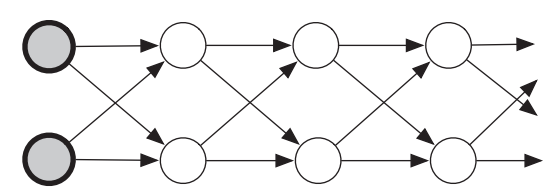
\includegraphics[width=0.5\linewidth]{images/narrow_network.png}
    \caption{A network where the disease must pass through a narrow structure of nodes. (source: \cite{networks})}
    \label{fig:narrow_network}
\end{figure}

Let $d$ be a disease with a high contagiousness of $p=0.8$ and infection period $t_I=1$. 
Using the assumptions made for calculating $R_0$ in the tree network this would result 
in $R_0 = 2 \cdot 0.8 = 1.6$ which indicates that the disease is relatively likely 
to never die out. Due to the structure of the network however, the disease is going to 
die out relatively quickly. The chance of the disease not spreading during a cycle is
$0.2^4=0.0016$ thus the disease will on average die out after $\frac{1}{0.0016}=625$ cycles.
This shows that in more complex networks the structure of the network also plays a big role
in the progression of the epidemic. It is not possible to calculate $R_0$ using just the
characteristics of the disease, the network structure also needs to be taken into account.
Knowing this it is impossible to accuarately calculate $R_0$ in a highly complex network.
It is however possible to observe the $R_0$ value during the epidemic for previous cycles.
Let $R_0^k$ be the $R_0$ value for cycle $k$ and $I_k$ the amount of infected nodes in cycle $k$.
Then $R_0^k = \frac{I_k}{I_{k-1}}$, with this the evolution of the $R_0$ value can be 
observed making it possible to estimate $R_0$ for future cycles and helping to understand
whether the disease is currently dying out ($R_0<0$) or not ($R_0>1$). A simulation can also
help to understand how the $R_0$ value of diseases will behave for a disease with certain 
quantities in a complex network.

\subsection{Limitations}
There are still some limitations to the SIR Model. Each person can only catch the disease at
most once and the model does not allow for simulating multiple diseases at the same time.
However the model allows most social networks to be represented, making it realtively easy
to extend this network to include more complex diseases with different levels of contagiousness
depending on the time a node has been infected or a non constant infection period.

\section{SIS Model}
The SIS Model is an extension to the SIR Model which also allows nodes to be reinfected multiple
times. The \textbf{R}emoved state is exchanged with the \textbf{S}usceptible state, so nodes
that are removed from the \textbf{I}nfected state are placed back in the \textbf{S}usceptible state.
With this change it is possible for diseases to last an inifinite time in a SIS Model in contrast
to an SIR Model where every simulation will end after a finite amount of steps after the 
disease burned through all nodes. The only way for the simulation in a SIS Model to end is
if all infected nodes fail to transmit the disease to any of their neighbors $t_I$ times.

\section{Custom Model}
\label{sec:custom_model}
\subsection{Parameters}
The model used by the developed app is a further extension to the SIR and SIS Models. It 
combines the SIR and SIS Model by having nodes that finish the infection period move either
into the \textbf{R}emoved or \textbf{S}usceptible state depending on a quantity $f$. Each
disease has a fatality rate $f$ which determines whether a node is moved into the 
\textbf{R}emoved state and considered deceased or moved back into the \textbf{S}usceptible
state if it survived the infection. The \textbf{S}usceptible state will be split into two
substates: nodes that never were infected before nad nodes that were put back into it after
being infected at least once. This allows for different infectiousness values $p_I$ for the
first infection of a node and $p_r$ for reinfections. 

The $t_I$ parameter will be split into two new parameters $t_{min}$ the minimum time an infection takes
before the node can be cured and $t_\rho$ the probability a node is cured from its infection
after the minimum time $t_{min}$ has elapsed. This results in four states so far:

\begin{itemize}
    \item Healthy: Susceptible nodes that were never infected before. They are at risk of being
    infected by their neighbors with a probability of $p_I$
    \item Infected: Nodes that are currently infected. The infection duration is least $t_{min}$ cycles and
    the exact duration is determiend by the probability $t_\rho$. After the infection ended the
    node is moved into the cured state with probability $1-f$ or into the deceased state with
    probability $f$.
    \item Cured: Nodes that were infected but survived. They are at risk of being
    infected by their neighbors with a probability of $p_r$ 
    \item Deceased: Nodes that died from the infection. They are not considered in future cycles
    and can not infect others anymore.
\end{itemize}

The infectiousness of a disease usually changes over the duration of the infections. In most
cases an infected person is most likely to infect other during the first few days of contracting
a disease. This should also be represented in the custom model. Thus the $p_I$ and $p_r$ values
need to change with the time a node has been infected $t_c$. These time dependant probabilities
will be called $p_I^t$ and $p_r^t$. A healthy node now has a probability of $p_I^t$ to
be infected by another node that is infected since $t$ cycles. Analogue a cured node 
now has a probability of $p_r^t$.

Another part of epidemics that is not represented in the SIR or SIS Model is vaccines.
During the course of an epidemic vaccines may be used which decrease the fatality rate
for infected persons and decrease the likelyhood for vaccinated person to be infected with
the disease. To incorporate this in the custom model two new states for nodes are added:
\begin{itemize}
    \item Vaccinated: Nodes that are vaccinated and now have a probability of getting infected
    of $p_v^t$ and a fatality rate of $f_v$.
    \item Unvaccinated: Nodes that are not vaccinated and use the above mentioned probabilities
    $p_I^t$/$p_r^t$ and $f$.
\end{itemize}
These two new states are not exclusive with the previous four states. Each node simultaneously
has one of the two states, vaccinated or unvaccinated, and one of the previous four states 
healthy, cured, infected or deceased.

\subsection{Network model}
The network model is very similar to the one used by the SIR and SIS Model. However it does
not allow for directed connections as there are very limited uses for those connections. 
Almost every human contact is bidirectional if for example one person gets close enough to
another person to contract an air transmitted disease this transmission can always happen
in both directions.

The network model used in this custom model organizes the nodes of one social circle in groups
to more clearly organize the network for more visual clarity. Each group can be 
considered a small-world %TODO ref
contact network were the nodes in each group are a localized part
of the network that is highly connected with fewer connections to other groups.

\section{Characteristics of epidemics}
\subsection{Oscillating diseases}
As explained by Easley and Kleinberg \cite{networks} diseases with certain characteristics
can cause an oscillating amount of infection. Consider a network with multiple highly
connected groups that have only have a few connections between the groups. If a disease
with a very high infection probability $p\geq0.9$, a period of immunity $i > 0$ and a
fatality rate close to zero breaks out in such a network, the infection amount will osciallate.
An example how the number of infections could evolve over time can be seen in figure 
\ref{fig:oscillation}.
\begin{figure}
    \centering
    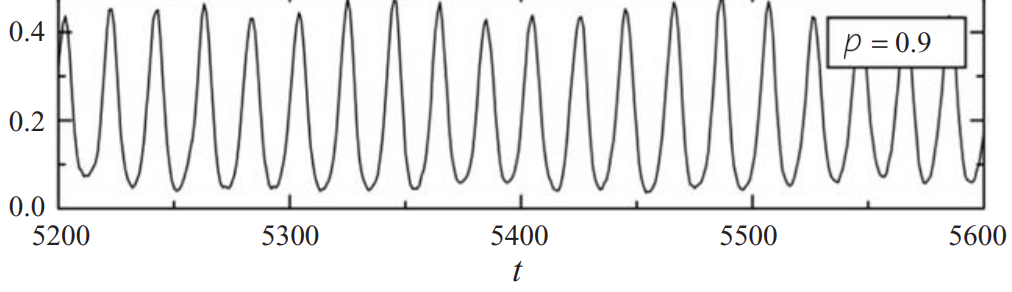
\includegraphics[width=0.5\linewidth]{images/oscillation.png}
    \caption{Amount of infections over time in a network of highly connected 
    groups. The disease has a high infection rate and low fatality. (source: \cite{networks})}
    \label{fig:oscillation}
\end{figure}

This happens because due to the high infectiousness of the disease almost all nodes of 
a group that has at least one infected node will be infected within a few cycles. Because
almost all nodes are infected after only a few cycles there are only a few new infections 
in the next cycles because of the sparse set of available healthy nodes. If the initial
wave started at cycle $c$ then at cycle $c' = c + t_i + i$ the nodes of the first wave 
are susceptible to infection again. Thus the amount of possible targets for new infections
increases drastically which causes the new infections to also rise again. This results in 
the oscillation of the amount of new infections.

Such a scenario can be modeled with the created tool. The network consists of 5 groups of 2,000 nodes
each having a lot of inner group connections (5 per node) and only a small amount of connections to the
other groups. Each group is connected to two other groups with 1 edge per node and it is ensured that
all groups have a connection to all other groups.

The disease that will be simulated in this network has a infection rate of 0.2, a fatality
rate of 0, a infection duration of 5 cycles and a immunity period of 3 cycles. For simplicity
the reinfection rate is the same as the initial infection rate and no vaccinations are used.

\begin{figure*}
    \centering
    \begin{subfigure}[b]{0.475\textwidth}
        \centering
        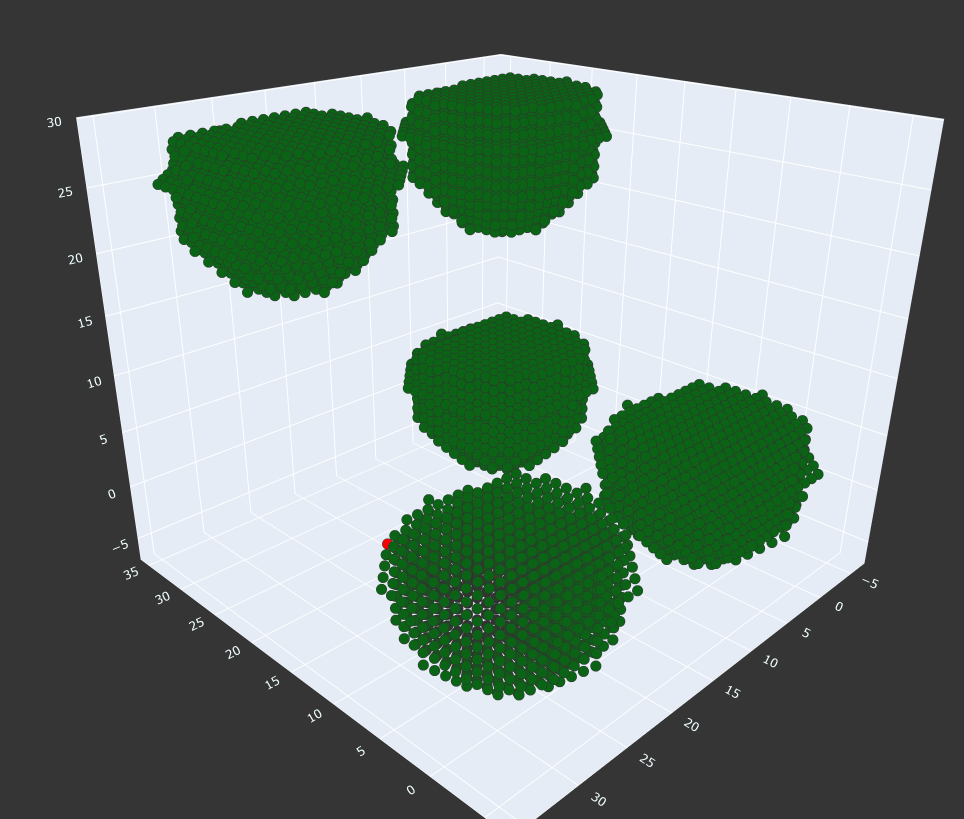
\includegraphics[width=\textwidth]{images/oscillation0.png}
        \caption[Network2]%
        {{\small Network after 0 Steps}}    
        \label{fig:mean and std of net14}
    \end{subfigure}
    \hfill
    \begin{subfigure}[b]{0.475\textwidth}  
        \centering 
        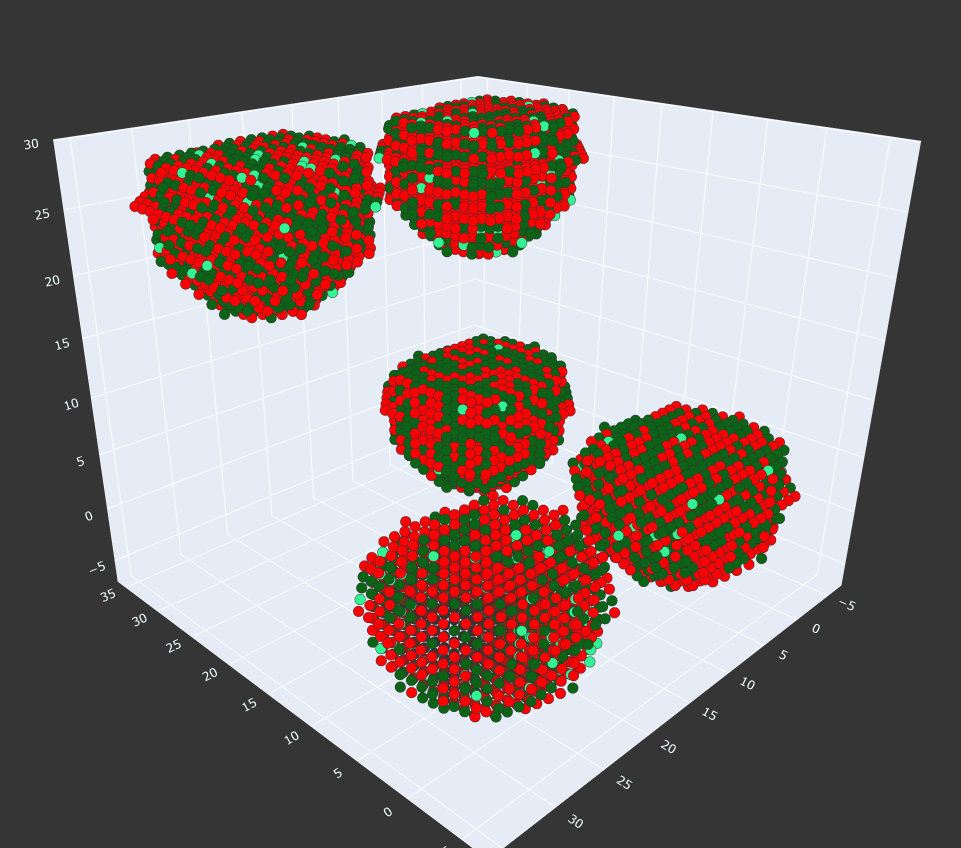
\includegraphics[width=\textwidth]{images/oscillation12.png}
        \caption[]%
        {{\small Network after 12 Steps, infections are at a maximum}}    
        \label{fig:mean and std of net24}
    \end{subfigure}
    \vskip\baselineskip
    \begin{subfigure}[b]{0.475\textwidth}   
        \centering 
        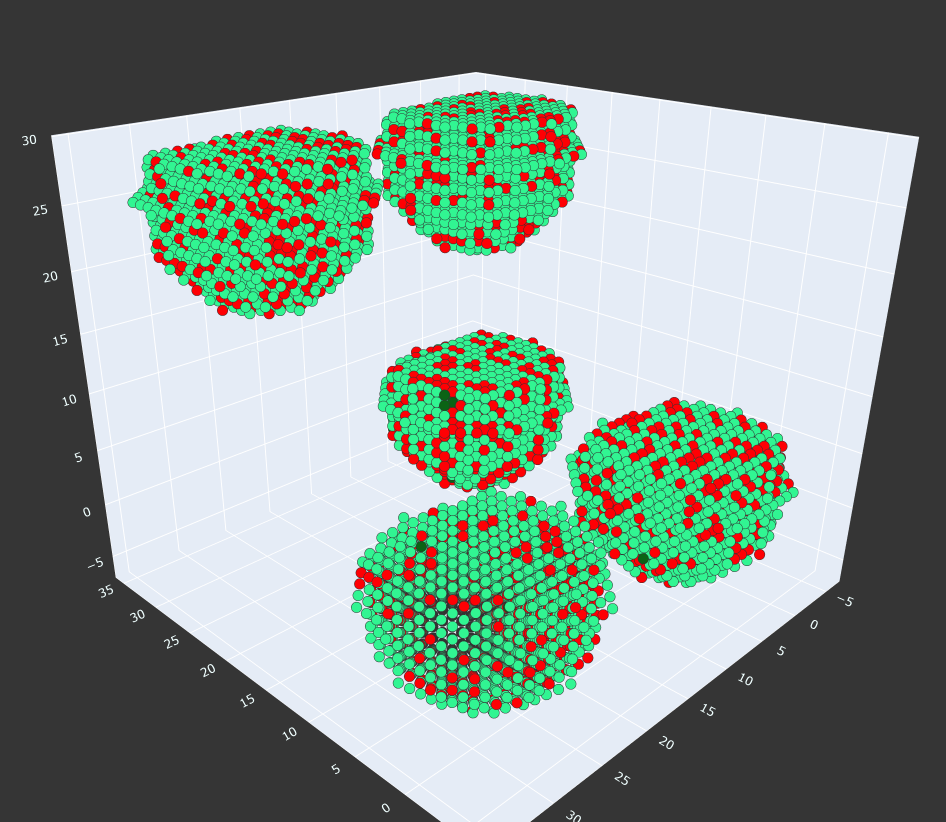
\includegraphics[width=\textwidth]{images/oscillation18.png}
        \caption[]%
        {{\small Network after 18 Steps, infection are at a minimum}}    
        \label{fig:mean and std of net34}
    \end{subfigure}
    \hfill
    \begin{subfigure}[b]{0.475\textwidth}   
        \centering 
        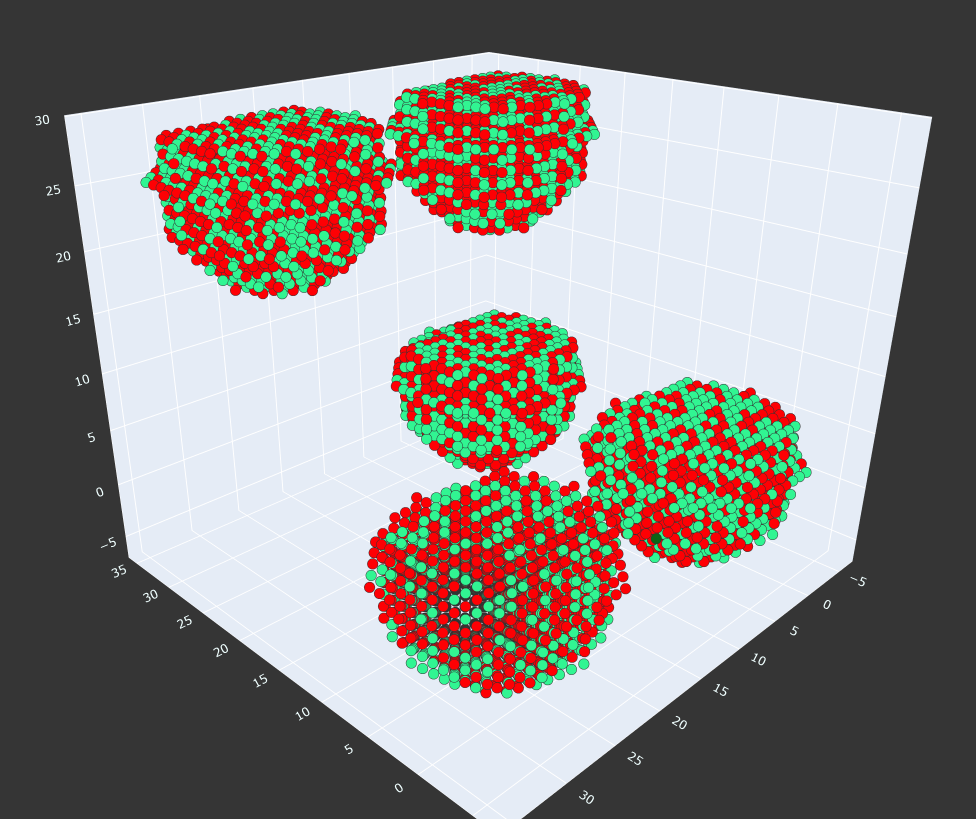
\includegraphics[width=\textwidth]{images/oscillation24.png}
        \caption[]%
        {{\small Network after 24 Steps, infection are at a maximum again}}    
        \label{fig:mean and std of net44}
    \end{subfigure}
    \caption[ State of the network showing the oscillation of infected nodes ]
    {\small State of the network showing the oscillation of infected nodes. Red nodes are currently infected, dark green ones have never been infected and 
    light green ones were previously infected but have recovered and have immunity.} 
    \label{fig:osc_network}
\end{figure*}

Initially 2 random nodes will be infected with the disease. Figure \ref{osc_network}
shows the state of the network after 0, 12, 18 and 24 cycles.
The amount of infections over time can be seen in figure \ref{fig:oscillation_p02}
which clearly shows the oscillating nature of this disease. Over time the amplitude of the
waves decreases, as the amount of people infected at the same time and thus getting cured
at the same time decreases so the infections are no longer synced and each cycle the same
amount of new nodes that can be infected becomes available. This happens because the
infection rate was too low. The disease was not able to explosively infect all new nodes
as soon as they became available which is why some nodes stayed uninfected for 2-3 cycles
thus shifting their cure time and breaking the oscillation. Increasing the infection rate
to $p = 0.3$ prevents this as now the disease spreads fast enough to instantly infect each
available node. The result of this is shown in figure \ref{fig:oscillation_p03}.

\begin{figure}
    \centering
    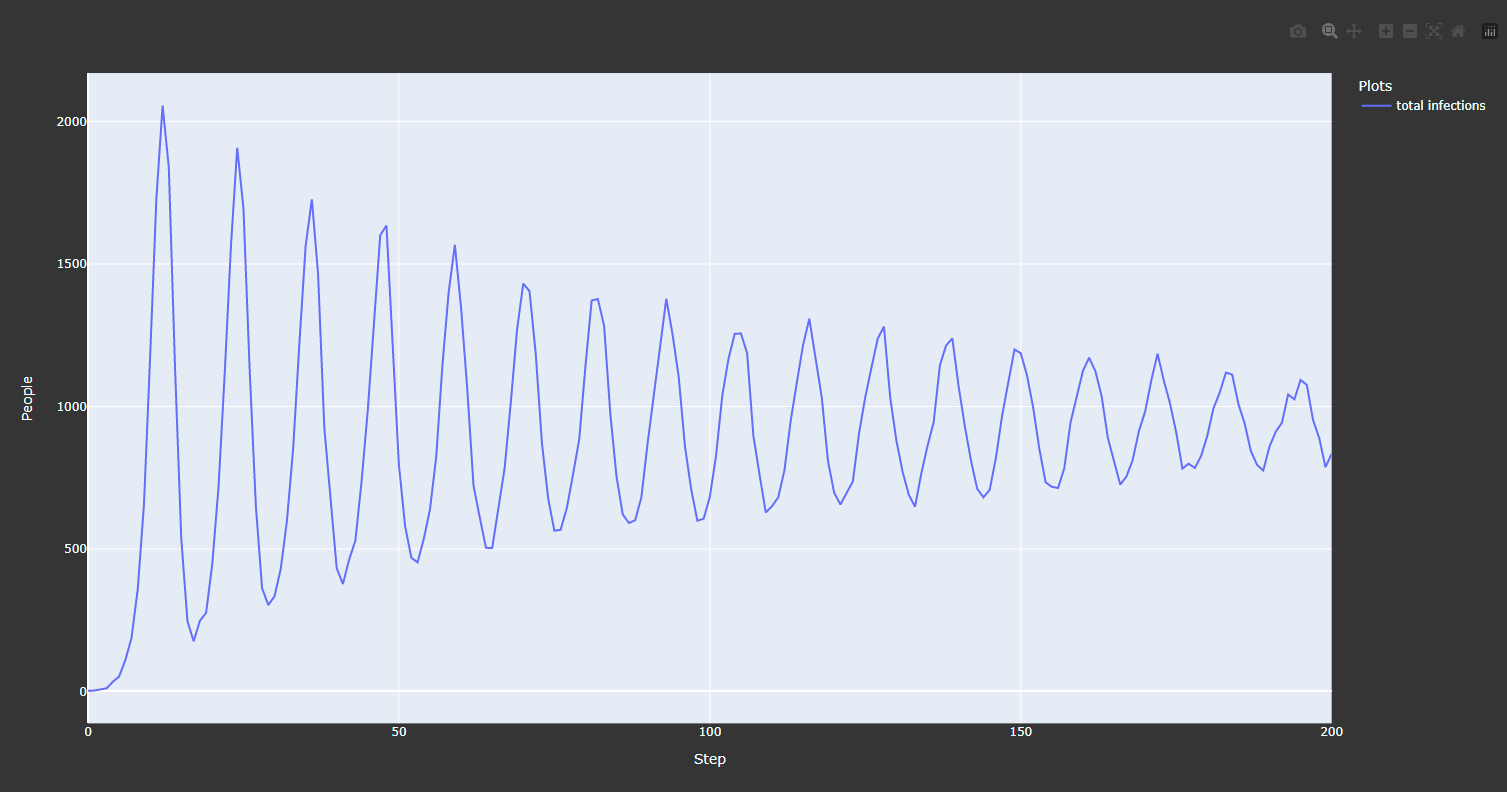
\includegraphics[width=0.5\linewidth]{images/oscillation_infections.png}
    \caption{Amount of infections over time showing the oscillating nature with $p = 0.2$}
    \label{fig:oscillation_p02}
\end{figure}

\begin{figure}
    \centering
    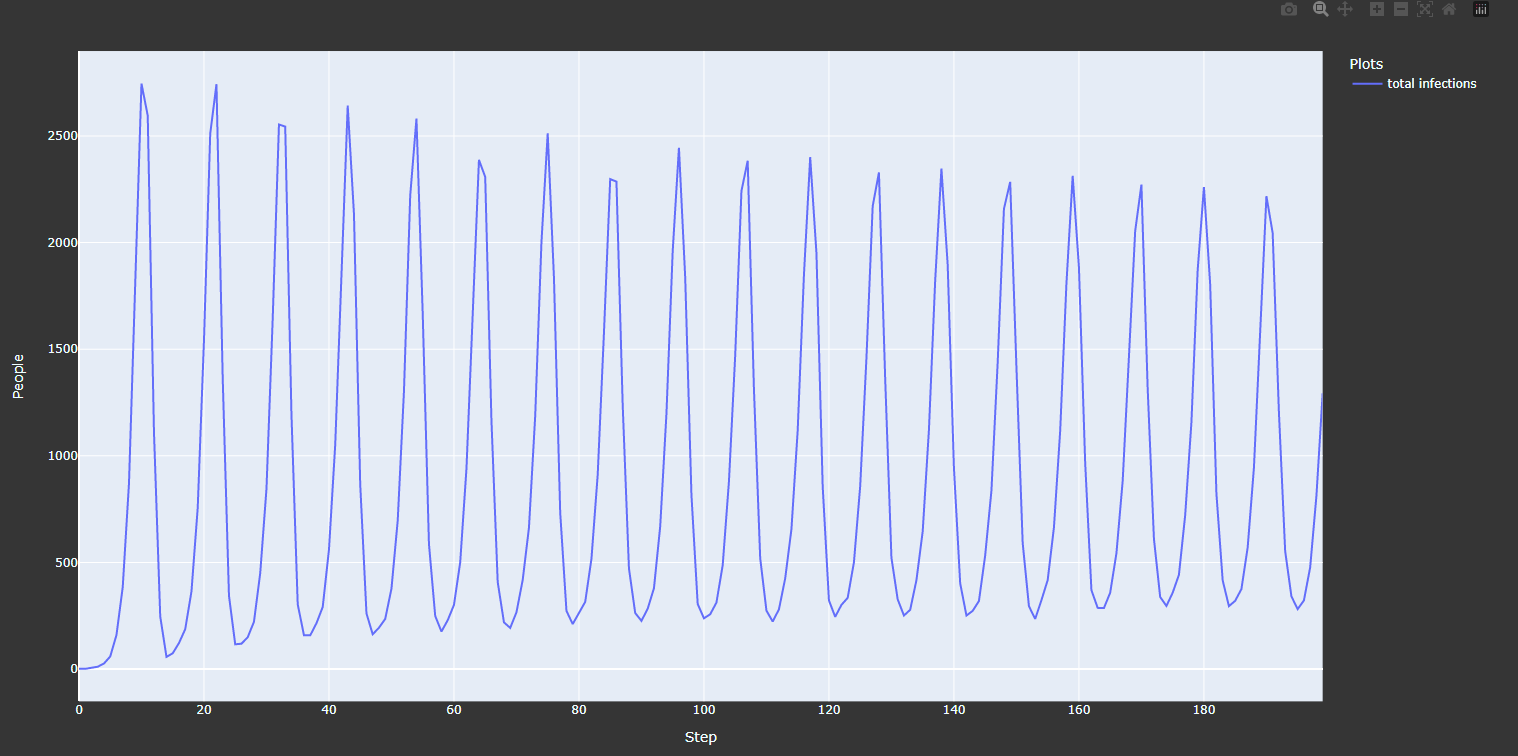
\includegraphics[width=0.5\linewidth]{images/oscillation_infections3.png}
    \caption{Amount of infections over time showing the oscillating nature with $p = 0.3$}
    \label{fig:oscillation_p03}
\end{figure}

Now the same network is used but the infection rate of the disease is decrease to 0.1.
Because the desease is now not spreading as explosively as before it always has enough targets
to infect until the previously infected nodes become cured again. Thus the amount of new 
infections is more consistent as seen in figure \ref{fig:no_oscillation}.

\begin{figure}
    \centering
    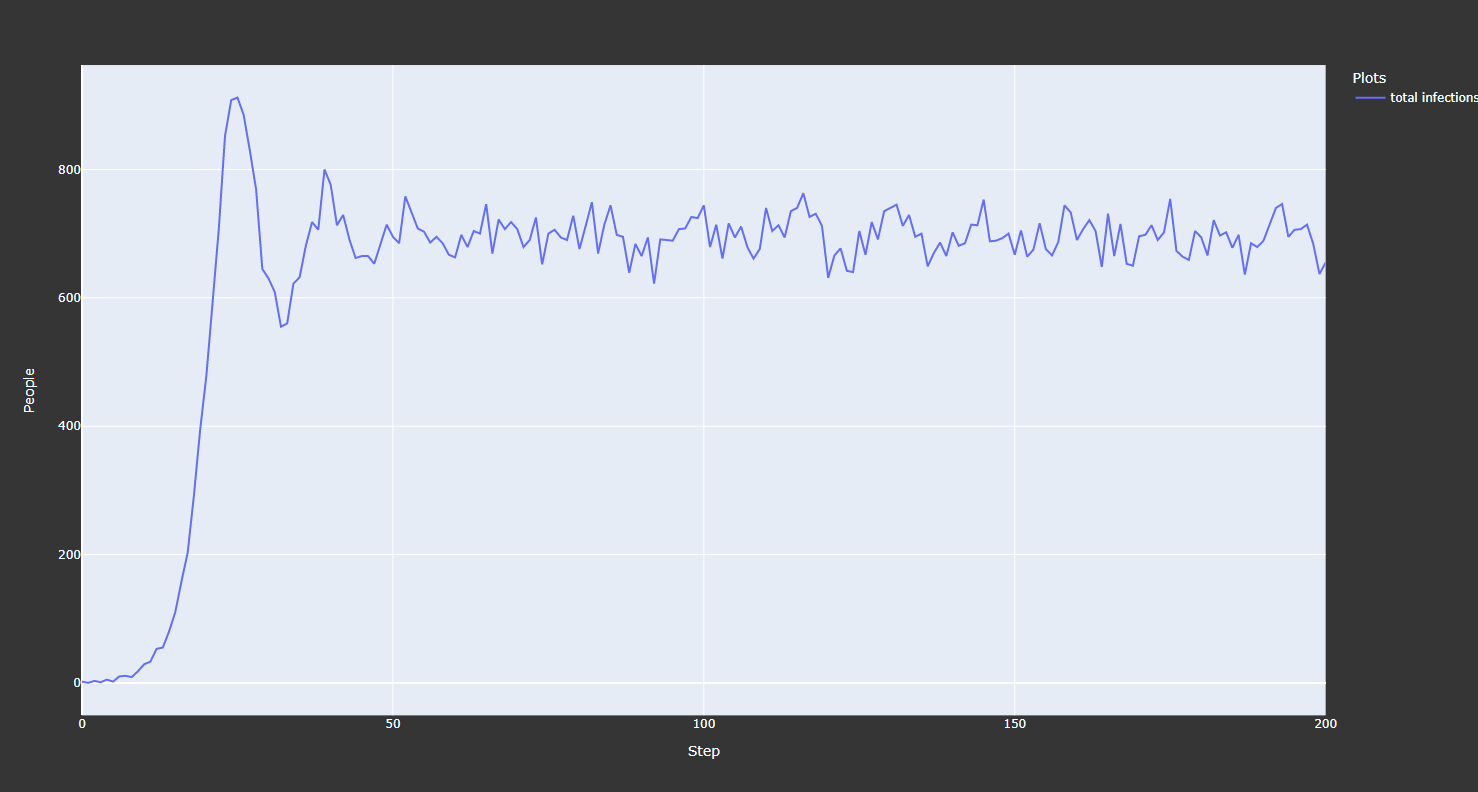
\includegraphics[width=0.5\linewidth]{images/no_oscillation.png}
    \caption{Amount of infections over time showing that no oscillations occur if with $p = 0.1$}
    \label{fig:no_oscillation}
\end{figure}

Another way to break the oscillation is to keep $p=0.3$ but decrease the duration of the infection to 2 cycles 
and remove the immunity period. Now the infected nodes become cured so fast that there are
enough new nodes to infect for every cycle thus again resulting in a relatively consistent
amount of new infections as indicated in figure \ref{fig:no_oscillation2}

\begin{figure}
    \centering
    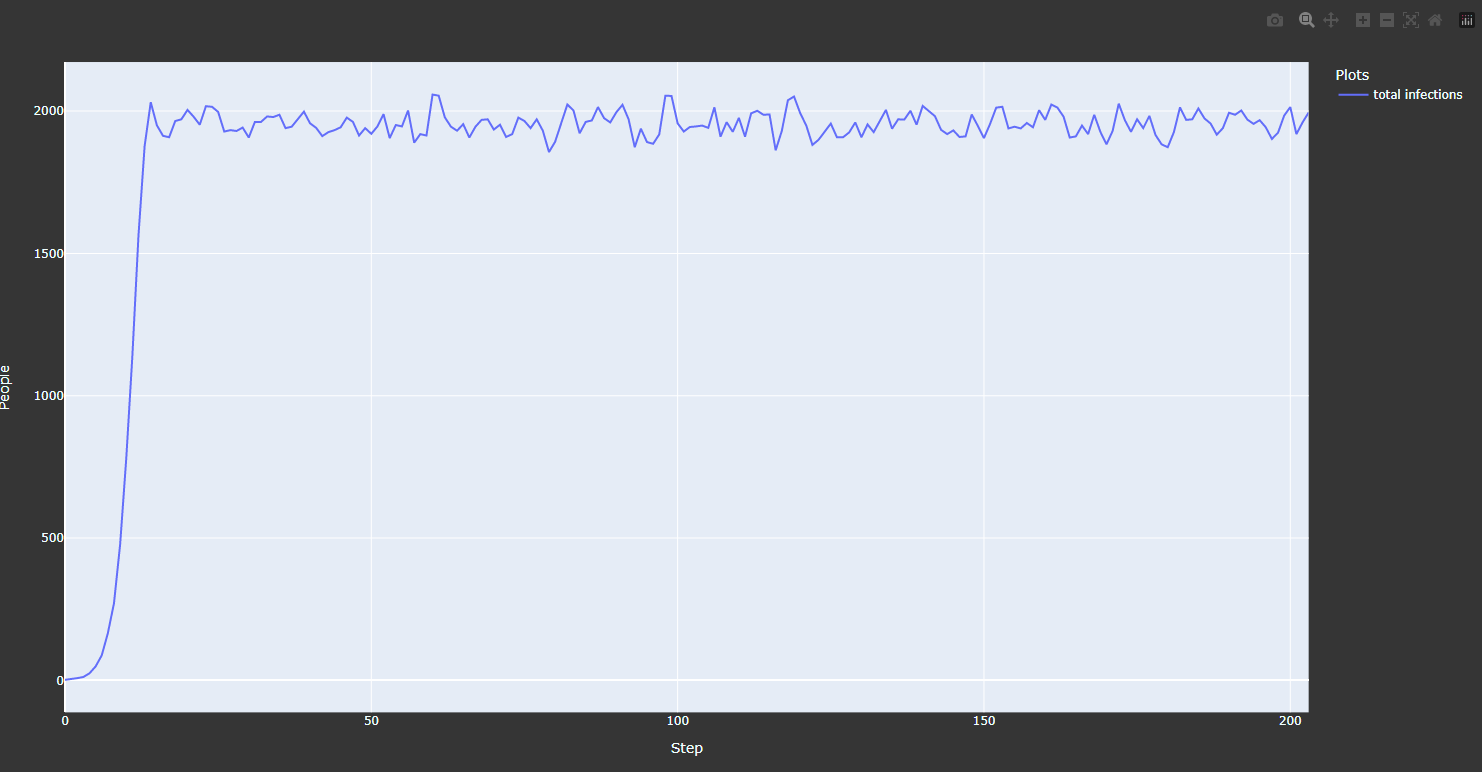
\includegraphics[width=0.5\linewidth]{images/no_oscillation2.png}
    \caption{Amount of infections over time showing that no oscillations occur even with $p = 0.3$ if the duration is too short}
    \label{fig:no_oscillation2}
\end{figure}

\subsection{Epidemics without diseases}
Diseases are not the only thing that is capable of spreading through social networks. As
previously mentioned computer viruses spread in a similar pattern. However there are other
completely different things that can spread in social networks in a similar way.
Information for example can be modeled using a very similar approach to the one proposed
for diseases. Information can be passed from person to person whenever they talk to each other
be that over a long distance through things like text messages or by meeting in person.

Other things that can spread through social networks include traditions or certain habits.
Looking at the world people within each country come into contact with other people from the
same country much more frequently than with people from other countries. This means each
country can be modeled as a highly connected group of people with few connections to other
countries. This model can be used to explain how each country has its own traditions that
differ from other countries the further away they are. Traditions spread easily within 
a country but the further away a country is the less likely the tradition is to spread to it.
As there are only few connections to other countries foreign traditions which only spread there
rarely are drowned out by the explosively spreading regional traditions of the country.

These models can also be used to model genetical inheritance. As suggested by
Easley and Kleinberg \cite{networks} this can be done by connecting parents to their offspring.
Then simulations can be run to show the spreading of different genetical factors throughout
the ancestry trees. This type simulation itself offers a lot of areas that can be expanded
on to create various simulations relevant to understanding human history and origin. 
It can also be used to indicate and visualize the existance of common ancestors and 
can give an idea of how many generations it takes to reach those. One such model that deals
with genetics and common ancestors is the Wright-Fisher Model. Haller and Messer \cite{genetics}
go into more detail how this model and the genetic simulation works. Genetic simulations 
and the Wright-Fisher Model are a big research area themselfes there are various other
works that talk about those topics, explaining the mathematics behind those models, 
possible uses etc. \cite{genetics2} \cite{genetics3} \cite{genetics4}.


This shows how the use of epidemics and social networks goes way beyond just diseases and
can help us understand complex relations in various different areas of research.

\chapter{Implementation}
\label{cha:implementation}
An app that allows for the simulation of epidemics is created. First the required functionalities
of the app need to be determined. It must be able to simulate different epidemics cases for
which different social networks and diseases are required.

\subsection{Network Editor}
The app needs an editor that allows for the creation of different social networks. Since
social networks can consist of a huge amount of people this editor needs to allow the user
to quickly create networks with a high amount of nodes and connections. For this there
will be three settings for a group of nodes:

\begin{itemize}
    \item \textbf{Size}: The amount of nodes in the group
    \item \textbf{Intra group connections}: The amount of edges each node has to other nodes
    of the same group
    \item \textbf{Intra group connections delta}: The variation for the amount of edges each
    node has ot other nodes of the same group. Eg. a connection amount of 5 with a delta of 3
    would result in each node having between 2 and 8 connections.
\end{itemize}

A network then consists of any amount of groups each with different settings. To allow
for connections between these groups there are similar settings availabe for each pair of
groups:

\begin{itemize}
    \item \textbf{Inter group connections}: The amount of edges each node has to other nodes
    of the other group
    \item \textbf{Inter group connections delta}: The variation for the amount of edges each
    node has ot other nodes of the other group. Eg. a connection amount of 5 with a delta of 3
    would result in each node having between 2 and 8 connections.
\end{itemize}

Using these properties the user is able to quickly generate big networks to model most
social situations. To visualize the structure of the network there will also be a 3D view
of the current network which can be updated after each change. Chapters \ref{cha:network_generation}
and \ref{cha:network_display} explain the implementation of this feature in more detail.

\subsection{Disease Editor}
To create the diseases that spread in the network the app has a tab were the required properties
for each diseases can be set. These include the properties discussed for the custom model in
section \ref{sec:custom_model} as well as some other properties required for visualizing the network:
\begin{itemize}
    \item \textbf{Name}: Name of the disease, will be shown in the legend when displaying the network
    \item \textbf{Color}: Color nodes infected with this disease will have
    \item \textbf{Fatality rate}: $f$, the chance a node is moved into the deceased state after the infection period is over
    \item \textbf{Vaccinated fatality rate}: Fatality rate for vaccinated nodes
    \item \textbf{Infection rate}: $p_I$, the chance an unvaccinated node gets infected by a neighbor
    \item \textbf{Reinfection rate}: $p_r$, the chance a previously infected node gets infected again by a neighbor
    \item \textbf{Vaccinated infection rate}: $p_v$, the chance a vaccinated node gets infected by a neighbor
    \item \textbf{Minimum duration}: $t_{min}$, the minimum cycles an infection lasts
    \item \textbf{Cure chance}: $t_\rho$, chance a node gets cured (or dies) each cycle after it has been
    infected for $t_{min}$ cycles
    \item \textbf{Immunity period}: Amount of cycles a node is immune after being cured
    \item \textbf{Infectiousness factor}: Decrease of infection rates with each cycle the node has been infected.
    Eg. with a initial $p_I = 0.5$ and a factor $I = 0.9$ the infection rate after $x$ cycles is $p = p_I \cdot I^x$.
    \item \textbf{Initial infections}: Amount of nodes infected with this disease in cycle 0, the start of the simulation
\end{itemize}

\subsection{Simulation}
To simulate diseases the app contains two different tabs. One where the network is displayed
in 3D and the current state of each node is indicated by colors. The other tab only contains
text for each group showing how many nodes are infected, deceased, etc. per group. The simulation
without visually seeing the graph allows for faster simulation of a high amount of steps and for
networks with a high amount of nodes (over 100,000, depends on computing power of the system)
building the graph might take a long time making the simulation with the visual representation
almost unusable.

Both simulations contain buttons to advance one step, automatically advance steps over time,
reset the simulation and save the statistics collected during the simulation. The simulation
which displays the networks also contains buttons to alter the display of the network, eg. to hide
certain node groups or edges to allow viewing only the areas of the network the user wants to observe.
Chapter \ref{cha:visual_simulation} explains the implementation of this feature in more detail.

\subsection{Statistics}
The last tab of the app can be used to view the statistics collected during simulations.
It displays the individual stats in a coordinate system and contains functions to split
the stats by different parameters, eg. show only infections with a certain disease or all
diseases or of only a certain group. The graph can be viewed as the individual value of each
step as well as the cumulative value up to each step.

\subsection{Frameworks}
The app is constructed using python. For the UI QT \cite{qt} is used, this is further explained
in chapter %TODO
For the display of the graphs the plotly \cite{plotly} is used along with the dash implementation
it provides for creating webpages. The graphs will then be displayed on the dash webpage
which is embedded in the QT app. The implementation of the website is explained in chapter %TODO.
For saving a project the JSON file format is used. The saved project files contain all 
necessary information, like the groups of the network, diseases and stats of previous simulations
to allow closing the app after saving without losing any progress.


\chapter{Network Generation}
\label{cha:network_generation}
The developed tool provides a user interface for generating networks to simulate epidemics. To create these networks, different groups of people can be defined. Each group consists of $n$ nodes, the members, each of which has a certain number of edges to other nodes of the same group. The number of edges per node is determined by a mean $\mu$ and a delta $\delta$. Each node will then have an edge count between $\mu - \delta$ and $\mu + \delta$.

Let $g1$ and $g2$ be two different groups. Then in addition to the above mentioned edges within a group, it is also possible to specify the number of edges between the nodes of the two groups with an average and delta value, in the same way as described above.

To create a network graph that meets all of these requirements multiple algorithms are needed.

\section{Creating edges within a group}
\label{sec:creating_edges_in_group}
Let $g$ be a group of $n$ nodes, each of which needs between $\mu - \delta$ and $\mu + \delta$ edges. Then the first step is to generate a sequence of $n$ integer numbers within this range. This sequence represents the degree each node should have at the end.

\subsection{Randomly adding new edges}
\begin{algorithm}
\caption{Adding random edges}
\label{alg:random_edges}
\begin{algorithmic}
\State $nodes \gets $nodes with less than required degree
\While{$nodes$ is not empty}
    \State $n1, n2 \gets$ two unconnected nodes
    \State connect $n1$ and $n2$
    \If {$n1$ has required degree}
        \State remove $n1$ from $nodes$
    \EndIf
    \If {$n2$ has required degree}
        \State remove $n2$ from $nodes$
    \EndIf
\EndWhile
\end{algorithmic}
\end{algorithm}

This algorithm was the first iteration for creating the networks, it has two issues. 
\newline

First, not every sequence of degrees is graphic, e.g. not every sequence of degrees has a corresponding simple graph. A simple graph is a graph consisting only of undirected edges and no loops.

For example, let $s$ be a sequence of random integers with sum $m$. If $m$ is not even, $s$ is definitely not graphic, because in a simple graph without loops, every edge increases the total degree of all nodes by two. Thus it is impossible to have a total degree of all nodes that is not even. This is not checked in the above algorithm \ref{alg:random_edges}, which would cause the $nodes$ list to contain only one node at the end, making it impossible to select two unconnected nodes from it.
\newline

The second issue is that by adding edges randomly it is possible to end up in a situation, where all remaining edges are already connected but have still not reached the required degree.

\begin{figure}
    \centering
    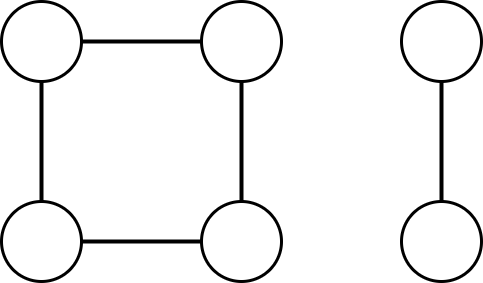
\includegraphics[width=0.5\linewidth]{images/impossible_graph.png}
    \caption{Graph created by random algorithm \ref{alg:random_edges} with $\mu=2$ and $\delta=0$}
    \label{fig:impossible_graph}
\end{figure}

Figure \ref{fig:impossible_graph} shows one such situation. In this graph each node needs to have a degree of exactly two. In theory it is possible to create such a graph, but the random algorithm \ref{alg:random_edges} may end up in the situation shown in the figure. Here the only two nodes remaining in the $nodes$ list are the two on the right which are already connected. From this state it is impossible to create a graph that satisfies the degree requirements.
\newline

The second iteration of the algorithm uses a more methodical approach to adding the edges to solve the above issues.

\subsection{Erdos-Gallai Theorem}
To solve the first problem of degree sequences that are not graphic, the Erdos-Gallai Theorem is used. It provides one of the two known approaches to solving the graph realization problem, i.e. it gives a necessary and sufficient condition for a finite sequence of natural numbers to be the degree sequence of a simple graph.

\begin{equation}
\sum_{i=1}^{k} d_i \leq k(k-1) + \sum_{i=k+1}^{n} \min(k, d_i)
\end{equation}
for all integers \(k\) with \(1 \leq k \leq n\), where \(d_1 \geq d_2 \geq \ldots \geq d_n\) are non-negative integers.

A sequence of degrees is graphic if and only if \(d_1 + d_2 + \ldots + d_n\) is even and the above equation holds for every $k$. The inequality ensures that the sum of the first $k$ terms of the degree sequence does not exceed the theoretical maximum number of edges $(k(k-1))$ plus the sum of the remaining edges $\sum_{i=k+1}^{n} \min(k, d_i)$ for the remaining vertices.

For this tool, every degree sequence needs to be graphic, because it should always be possible to generate a graph for the user's input. This means that if the Erdos-Gallai Theorem shows that a sequence is not graphic, it must be changed until it is. This is done by simply decrementing a random number of the degree sequence by one.

If the Erdos-Gallai Theorem failed because the sum was not even, the sum will be even after decrementing once. By decrementing random numbers of the sequence, only the left side of the inequality gets smaller, because $k$ never changes. This means after decrementing enough times, the theorem will always be fulfilled. Thus, any sequence of degrees can be changed to be graphic.

The python implementation of this algorithm can be seen in \ref{lst:erdos_gallai}.

\begin{lstlisting}[language=python, caption={Erdos-Gallai Theorem in Python}, label={lst:erdos_gallai}]
def _erdos_gallai(self) -> bool:
    if sum(self.deg_seq) % 2 != 0:
        return False
    n = self.size
    for k in range(1, n + 1):
        if sum(self.deg_seq[:k]) > k * (k - 1) + sum(min(k, d) for d in self.deg_seq[k + 1 :]):
            return False
    return True
\end{lstlisting}

\subsection{Havel-Hakimi algorithm}
\label{sub:havel_hakimi}
After creating a graphic degree sequence using the Erdos-Gallai Theorem, with all degrees within the $\mu - \delta$ and $\mu + \delta$ range, this degree sequence needs to be converted to a network graph.

\begin{algorithm}
\caption{Havel-Hakimi algorithm}
\label{alg:havel_hakimi}
\begin{algorithmic}
\State $deg\_seq \gets $ graphic sequence of degrees
\State $nodes \gets $ list of nodes, with same length as $deg\_seq$
\While{$sum(deg\_seq) > 0$}
    \State $n \gets nodes.pop(0)$
    \State $d \gets deq\_seq.pop(0)$
    \State $targets \gets $ n nodes with highest degree from $nodes$
    \For{$t$ in $targets$}
        \State connect $t$ and $n$
        \State $deg\_seq[t] \gets deg\_seq[t] - 1$
    \EndFor
\EndWhile
\end{algorithmic}
\end{algorithm}

Using the Havel-Hakimi algorithm \ref{alg:havel_hakimi} a simple graph can be constructed for every graphic sequence of degrees. This algorithm always finds a correct solution as proven by Erdős et al. \cite{havelHakimi}.

\subsubsection{Python implementation}
The Havel-Hakimi algorithm is implemented in the class HavelHakimi. This class has properties for the sequence of degrees \texttt{deg\_seq}, list of node ids \texttt{node\_id\_seq} and a dictionary which nodes are connected \texttt{edges} (each key node id has an undirected edge to all its value node ids).

First the \texttt{node\_id\_seq} is sorted to be non-increasing and the \texttt{node\_id\_seq} is shuffled to assign random degrees to each node. Then the Havel-Hakimi algorithm is used:

\begin{lstlisting}[language=python, caption={Havel Hakimi Algorithm in Python}, label={lst:havel_hakimi}]
def _connect_nodes(self):
    while sum(self.deg_seq) > 0:
        node = self.node_id_seq.pop(0)
        deg = self.deg_seq.pop(0)
        targets = self._get_highest_n_nodes(deg)
        for target in targets:
            self.deg_seq[self.node_id_seq.index(target)] -= 1
        self.edges[node] = targets
        self._sort_sequence()
\end{lstlisting}

The function in listing \ref{lst:havel_hakimi} implements the above algorithm \ref{alg:havel_hakimi}. After each iteration, the degree sequence is sorted so it is non-increasing again. When sorting the \texttt{deg\_seq} it is important that the \texttt{node\_id\_seq} is altered in the same way so each node id still corresponds to the same degree, this function is shown in \ref{lst:sorting}.

\begin{lstlisting}[language=python, caption={Sorting degrees and node ids}, label={lst:sorting}]
def _sort_sequence(self):
    self.node_id_seq = [x for _, x in sorted(zip(self.deg_seq, self.node_id_seq), reverse=True)]
    self.deg_seq.sort(reverse=True)
\end{lstlisting}

\section{Creating edges between groups}
Randomly creating edges between two groups leads to similar problems as described in section \ref{sec:creating_edges_in_group}. Therefore, a modified version of the Havel-Hakimi algorithm and the Erdos-Gallai theorem is used.

\subsection{Creating the degree sequence}
Let $g1$ and $g2$ be two disjoint groups of size $n$ and $m$. If $n \neq m$, it may not be possible for every node to have a degree between $\mu - \delta$ and $\mu + \delta$. Let $n = 5$ and $m = 10$ with $\mu = 5$, $\delta = 0$. If every node in $g2$ has a degree of $5$, all nodes in $g1$ would have a degree of $10$. If every node in $g1$ has a degree of $5$, the average degree of the nodes in $g2$ would be only $2.5$.

So if $n \neq m$ one group may have lower degrees than the minimum or higher degrees than the maximum for certain $\mu$ and $\delta$. In this work the solution where the bigger group may have a lower degree will be used.
\newline

First, the degree sequence for the smaller group $g1$ is created. The sequence consists of $n$ integer numbers between $\mu - \delta$ and $\mu + \delta$. The degree sequence of the $g2$ must have the same sum as the sequence of $g1$, otherwise the sequences are not graphic because each added edge decreases the sum of the degree sequences of $g1$ and $g2$ by one and the Havel-Hakimi algorithm finishes only when both sequences reach $0$.
\newline

Let $s1$ be the sum of the degree sequence for $g1$. An algorithm is needed to generate a sequence of $m$ integer numbers with sum $s1$, where the numbers should be as close to or inside the desired range $\mu - \delta$ to $\mu + \delta$ as possible.

\begin{algorithm}
\caption{Sequence generation}
\label{alg:seq_with_sum}
\begin{algorithmic}
\Require {$(g1, m, g1\_deg\_seq, \mu, \delta$)}
\Ensure {$g2\_deg\_seq$}
\State $s1 \gets sum(g1\_deg\_seq)$
\State $seq \gets $ sequence of $m$ random integers between $\mu - \delta$ and $\mu + \delta$
\While{$sum(seq) != s1$}
    \If{$sum(seq) > s1$}
        \State $indices \gets []$
        \For {$deg$ in $seq$}
            \If{$deg > \mu - \delta$}
                \State $indices$ push $deg$
            \EndIf
        \EndFor
        \If{length of $indices$ == 0}
            \For {$deg$ in $seq$}
            \If{$deg > 0$}
                \State $indices$ push $deg$
            \EndIf
            \EndFor
        \EndIf
        \State $i \gets $ random entry of $indices$
        \State $seq[i] \gets seq[i] - 1$
    \Else
        \State $indices \gets []$
        \For {$deg$ in $seq$}
            \If{$deg < \mu + \delta$}
                \State $indices$ push $deg$
            \EndIf
        \EndFor
        \State $i \gets $ random entry of $indices$
        \State $seq[i] \gets seq[i] + 1$
    \EndIf
\EndWhile
\end{algorithmic}
\end{algorithm}

The algorithm \ref{alg:seq_with_sum} first generates a random sequence of integers in the range $\mu - \delta$ to $\mu + \delta$. If the sum of this sequence is too big, it decrements random entries until all degrees are equal to $\mu - \delta$. If this is still too large, random entries are decremented further until the required sum is reached. If the initial sum of the sequence is too small, random entries are incremented until the required sum is reached. It is always possible to reach the sum without any element of the sequence being greater than $\mu + \delta$, because the length of this sequence will always be smaller than or equal to the sequence of the first group. Thus, the maximum sum of the $g1_{seq}$ is $n \cdot (\mu + \delta)$ and the maximum sum of $g2_{seq}$ is $m \cdot (\mu + \delta)$. Since $n \leq m$ the following always holds: $n \cdot (\mu + \delta) \leq m \cdot (\mu + \delta)$. So the sequence of length $m$ generated by the algorithm \ref{alg:seq_with_sum} will never be bigger than the maximum of degrees within the range $\mu - \delta$ to $\mu + \delta$.

The python implementation of this algorithm is shown in listing \ref{lst:seq_with_sum}.

\begin{lstlisting}[language=python, caption={Algorithm for creating a sequence with specific sum}, label={lst:seq_with_sum}]
def _create_sequence_with_sum(self, size: int, _sum: int):
    seq: List[int] = np.random.randint(self.min_deg, self.max_deg + 1, size=(size)).tolist()
    while sum(seq) != _sum:
        if sum(seq) > _sum:
            if len(choices := [x for x in seq if x > self.min_deg]) == 0:
                choices = [x for x in seq if x > 0]
            seq[seq.index(random.choice(choices))] -= 1
        else:
            seq[seq.index(random.choice([x for x in seq if x < self.max_deg]))] += 1
    return seq
\end{lstlisting}

Since the second degree sequence is always constructed so that the two sequences together are graphic, the Erdos-Gallai Theorem is theoretically not needed here. It is still used to check the result in case there are any implementation errors that produce a non-graphic sequence, though it should always return true if the implementation has no problems. The modified implementation of the Erdos-Gallai Theorem can be seen in listing \ref{lst:modified_erdos_gallai}. This implementation tests the inequality for two sets of values: $n$, the size of $g1$, with $g2\_deg\_seq$ and $m$, the size of $g2$ with $g1\_deg\_seq$. This combination of values is used because the nodes of $g2$ have to be connected to the $n$ nodes of $g1$ and vice versa. If the second degree sequence is constructed using the above algorithm \ref{alg:seq_with_sum}, this function will always return true.

\begin{lstlisting}[language=python, caption={Modified Erdos-Gallai Theorem for connecting to disjunct groups}, label={lst:modified_erdos_gallai}]
def _erdos_gallai(self) -> bool:
    for n, seq in zip([self.size1, self.size2], [self.deg_seq2, self.deg_seq1]):
        for k in range(1, n + 1):
            if sum(seq[:k]) > k * (k - 1) + sum(min(k, d) for d in seq[k + 1 :]):
                return False
    return True
\end{lstlisting}



\subsection{Modified Havel-Hakimi algorithm}
The Havel-Hakimi algorithm from section \ref{sub:havel_hakimi} is modified to use two disjoint groups of nodes that it connects. The implementation of the modified algorithm can be seen in listing \ref{lst:modified_havel_hakimi}. Before this algorithm is used, the two degree sequences are constructed and sorted to be non-increasing. The two node id sequences are also created and shuffled.

\begin{lstlisting}[language=python, caption={Modified Havel-Hakimi algorithm}, label={lst:modified_havel_hakimi}]
def _connect_nodes(self):
    while sum(self.deg_seq1) + sum(self.deg_seq2) != 0:
        if self.size1 <= self.size2:
            node = self.node_id_seq1.pop(0)
            deg = self.deg_seq1.pop(0)
            targets = self._get_highest_n_nodes(deg, self.deg_seq2, self.node_id_seq2)
            for target in targets:
                self.deg_seq2[self.node_id_seq2.index(target)] -= 1
        else:
            node = self.node_id_seq2.pop(0)
            deg = self.deg_seq2.pop(0)
            targets = self._get_highest_n_nodes(deg, self.deg_seq1, self.node_id_seq1)
            for target in targets:
                self.deg_seq1[self.node_id_seq1.index(target)] -= 1
        self.edges[node] = targets
        self._sort_sequence()
\end{lstlisting}

The algorithm creates the edges starting from the smaller group. Let $d$ be the highest degree of the smaller group. Then a node from the smaller group with degree $d$ is selected for \texttt{node}. After that $d$ nodes with the highest degrees are selected from the list of nodes of the \textbf{other} (bigger) group. This is the main difference from the original Havel-Hakimi algorithm, which selects the nodes from the same group. Then the \texttt{node} from the smaller group is connected to each selected node from the larger group and the degrees for all nodes \texttt{node} is connected to are decremented.

\chapter{Network Display}
\label{cha:network_display}
Originally, it was intended to display the networks in 2D, with a 3D representation being considered a nice to have feature. During testing we found that a 2D representation does not provide a clear view of the network. Even for relatively small networks (\textasciitilde 200 nodes) the 2D representation was very confusing. For this reason, the 2D representation was scrapped and only the 3D one was implemented. In 3D, even networks with thousands of nodes provide a clear view of the different groups and nodes.
\newline

The Python package plotly \cite{plotly} is used to display the networks in 3D. \texttt{plotly.graph\_objs} provides the \texttt{Scatter3d} function, which is used to draw both the nodes and edges. For the nodes the function takes in three lists of coordinates, one for each axis x, y and z. For the edges it also requires these three lists, but here the first coordinate is the start point for an edge, the second the end point, followed by a None entry and then the next edge coordinates. Currently, the only information that is generated for graphs is the number of nodes in each group and lists of which node ids must be connected with edges. This information must be translated into coordinates for plotly to be able to display the network.

\section{Displaying the nodes}
\label{sub:displayNodes}
All nodes belonging to the same group should be arranged in a sphere. Each sphere thus represents one group and the spheres must have enough space between them so that the groups can be easily distinguished, as shown in Figure \ref{fig:groups}.

\begin{figure}
    \centering
    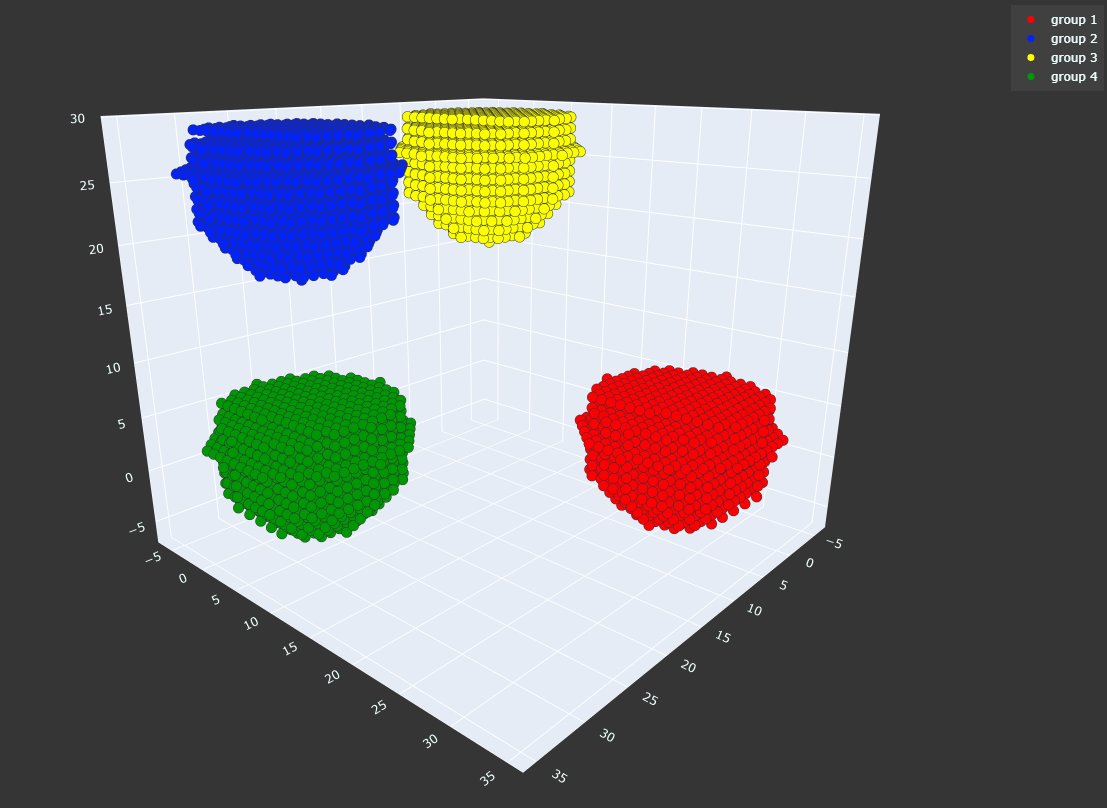
\includegraphics[width=0.75\linewidth]{images/groups.png}
    \caption{Network containing 4 groups with 2000 nodes per group}
    \label{fig:groups}
\end{figure}

To distribute the spheres in the coordinate system, it is first divided into cubes. Let $n_{max}$ be the number of nodes in the biggest group. To determine the side length $s$ of the cubes, it is necessary to know the radius $r$ of the smallest sphere that can fit $n_{max}$ nodes.

\subsection{Creating a sphere}
The nodes are placed only at coordinates $x,y,z \in \mathbb{N}$. To create a sphere that can fit $n_{max}$ nodes, the radius needs to be known before the exact coordinates are calculated. The problem with this is that the only way to get the exact radius for a sphere that can fit $n_{max}$ nodes that are all at coordinates $x,y,z \in \mathbb{N}$ is to use the algorithm depicted in \ref{alg:exact_radius}.
\begin{algorithm}
\caption{Calculating exact radius}
\label{alg:exact_radius}
\begin{algorithmic}
\Require {$(n_{max})$}
\Ensure {$r$}
\State $r \gets 0$
\State $n \gets 0$
\While{$n < n_{max}$}
    \State $r \gets r+1$
    \State coords $\gets$ calculate coordinates for all nodes in sphere with radius $r$
    \State $n \gets $ length of coords
\EndWhile
\end{algorithmic}
\end{algorithm}
This algorithm is inefficient because it computes all spheres until $r$ is big enough. This can be improved by estimating the number of nodes in a sphere of radius $r$ instead of computing the exact number. The number of nodes is estimated using the formula \ref{eq:sphere_lattice}.
\begin{equation}
\label{eq:sphere_lattice}
    \dfrac{4 \cdot \pi \cdot r^3}{3}
\end{equation}
This estimation incurs an error. \ref{eq:gauss_error} shows the best currently known formula for calculating this error which was discovered and proven by Zheng \cite{gaussSphereProblem}.
\begin{equation}
\label{eq:gauss_error}
    \sum_{\substack{x \in z^3 \\ |x| \leq r}}{P(x)} = O_{\epsilon, P}(r^{v + 84 / 63 + \epsilon})
\end{equation}
The true error bound is suspected to be $O_\epsilon(R^{1 + \epsilon})$ but this is currently not possible to prove. For the context of this work the simpler estimation shown in formula \ref{eq:gauss_error_rough} is sufficient.
\begin{equation}
\label{eq:gauss_error_rough}
    O_{\epsilon}(r^{21/16 + \epsilon})
\end{equation}

Let $r_e$ be the resulting radius required for $n_{max}$ nodes using the estimation. If $n_{max}$ is close to the boundary between two radii, then the resulting radius may be too large or too small due to the introduced error. For this reason, the resulting radius is decremented by one and the exact calculation is then used to find the correct required radius, as shown in algorithm \ref{alg:exact_radius_improved}. This will always find the smallest radius for a sphere containing at least $n_{max}$ points.

\begin{algorithm}
\caption{Calculating exact radius}
\label{alg:exact_radius_improved}
\begin{algorithmic}
\Require {$(n_{max})$}
\Ensure {$r$}
\State $r \gets 0$
\State $n \gets 0$
\While{$n < n_{max}$}
    \State $r \gets r + 1$
    \State $n \gets$ estimate amount of nodes in sphere with radius $r$
\EndWhile
\State $ r \gets r - 1$
\While{len(coords) $ < n_{max}$}
    \State coords $\gets$ calculate exact coords of nodes for radius $r$
\EndWhile
\end{algorithmic}
\end{algorithm}

The formula \ref{eq:sphere_inequality} represents the inequality for points inside or on the surface of a sphere centered at the origin in three-dimensional space, as proven by Gui and Moradifam \cite{sphereInequality}. A point is inside the sphere if this inequality is satisfied.
\begin{equation}
\label{eq:sphere_inequality}
    x^2 + y^2 + z^2 \leq r^2
\end{equation}
This means the bigger one of the values $x,y,z$ becomes, the smaller the other must be to satisfy the inequality. Using this knowledge, it is possible to construct an algorithm (shown in \ref{alg:calc_sphere_points}) that efficiently computes all triples of $x,y,z$ values that satisfy the inequality. The order of $z,x,y$ in the algorithm is important, so a half full sphere creates points that fill the sphere from the bottom to the top.
Starting with $z$ and $y=0$, transforming the formula to $x$ results in $|x| \leq \sqrt{(r^2 - z^2)}$, which corresponds to all possible values of $x$ with respect to $z$ and $r$. This range corresponds to $-a,a$ in the algorithm. Solving for $y$ then results in $|y| \leq \sqrt{(r^2 - z^2 - x^2)}$, which yields all possible values for $y$ with respect to $x,z,r$. This coincides with $-b,b$ in the algorithm.

\begin{algorithm}
\caption{Calculating lattice points}
\label{alg:calc_sphere_points}
\begin{algorithmic}
\Require {$r$}
\Ensure {$coords$}
\State $coords \gets []$
\For {$z := -r$ to $r$}
    \State $a \gets \lfloor\sqrt{(r^2 - z^2)}\rfloor$
    \For {$x := -a$ to $a$}
        \State $b \gets \lfloor\sqrt{(a^2 - x^2)}\rfloor$
        \For {$y := -b$ to $b$}
            \State coords $\gets (x,y,z)$
        \EndFor
    \EndFor
\EndFor
\end{algorithmic}
\end{algorithm}

The Python implementation of this function takes in an amount of points $n$ and returns a list of triples of length $n$ containing the resulting coordinates and the radius $r$ of the sphere.

\section{Arranging the spheres}
After calculating the coordinates and radii for each sphere (one for each group), the biggest radius $r_{max}$ is known. Using this, the side length of the cubes can be calculated. To create some space between the spheres, this side length $s$ is calculated as $s = 2 * r_{max} * 1.25$ to add an empty space of 12.5\% of the sphere diameter on each side.

The cubes are always created within a larger cube, e.g. the number of cubes is $c = x^3$. $x$ is the side length of the bigger cube in cubes (e.g. a side length of $x=3$ cubes results in $c=27$ smaller cubes). In order not to spread out the spheres unnecessarily, the smallest number of cubes should be created. The minimum required number of cubes is the number of spheres/groups. To get the next higher value for $c$, $x$ can be calculated by $x =\lceil\sqrt[3]{num\_groups}\rceil$.

Using this the algorithm \ref{alg:cube_offsets} computes the coordinates of bottom left corner of each cube.

\begin{algorithm}
\caption{Calculating cube offsets}
\label{alg:cube_offsets}
\begin{algorithmic}
\Require {$num\_group, r_{max}$}
\Ensure {$offsets$}
\State $s \gets \lceil 2 * r_{max} * 1.25\rceil$
\State $o \gets \lceil 2 * r_{max} * 0.125\rceil$
\State $c \gets \lceil\sqrt[3]{num\_groups}\rceil$
\For {$x,y,z := 0$ to $c$}
    \State offsets $\gets (x \cdot s + o, y \cdot s + o, z \cdot s + o)$
\EndFor
\end{algorithmic}
\end{algorithm}

For each sphere a random cube is selected and its offsets are added to the coordinates of all points within the sphere, resulting in the final coordinates for all nodes in the network.

\section{Creating the scatter graph}
\label{sub:scatter_graph}
In the final graph it must be possible to toggle the visibility of each group. To achieve this, the coordinates for each group are stored separately and only the active ones are added to the coordinate lists for the \texttt{Scatter3d} call.

\begin{lstlisting}[language=python, caption={Creation of the node trace}, label={lst:node_trace}]
for group in self.network.groups:
    if group.id not in self.hidden_groups:
        x, y, z = zip(*self.group_coords[group.id])
        aXn.extend(x)
        aYn.extend(y)
        aZn.extend(z)
        colors.extend([group.color] * len(x))
trace1 = go.Scatter3d(
    x=aXn,
    y=aYn,
    z=aZn,
    mode="markers",
    name="nodes",
    marker=dict(
        symbol="circle",
        size=6,
        color=colors,
        line=dict(color="rgb(50,50,50)", width=0.5),
    ),
    uirevision="0",
    showlegend=False,
)
\end{lstlisting}

The code in \ref{lst:node_trace} creates the trace that displays all active nodes. Whenever the visibility of a group is toggled, this trace must be rebuilt. It is important to note that the coordinates for the nodes in the x,y,z arrays contain the nodes in ascending order by their id. This means that nodes of group 0 come first starting with node 0, then group 1, and so on. This is important for creating color sequences based on the node states, which is discussed in section \ref{sec:color_sequence}.

\section{Displaying the edges}
The edges are displayed using a second \texttt{Scatter3d} with the \texttt{lines} mode. For this the x,y and z arrays need the format of [xStart, xEnd, None] for each line. This means that a coordinate array for 100 lines would have a length of 300.

The current format in which the edges are represented contains only the node ids that are connected by edges. This representation was created in section \ref{sub:havel_hakimi}. To translate these node ids to the coordinates of the nodes calculated in section \ref{sub:displayNodes}, a map is created when the coordinates are calculated for each node. This map stores the node id as a key and the index of its coordinates, in the coordinate array, as value. This map can be used to calculate the start and end coordinates for all edges of visible groups, which is done by looking up the coordinates of the start and end nodes by using their ids and the map. The python code that realizes this can be seen in listing \ref{lst:edge_creation}.
\begin{lstlisting}[language=python, caption={Creation of the edge coordinate arrays}, label={lst:edge_creation}]
 for edge in edges:
    _from, to = edge[0], edge[1]
    if not (_from in node_id_map and to in node_id_map):
        continue
    from_ind = node_id_map[_from]
    to_ind = node_id_map[to]
    aXe.extend([node_coords_x[from_ind], node_coords_x[to_ind], None])
    aYe.extend([node_coords_y[from_ind], node_coords_y[to_ind], None])
    aZe.extend([node_coords_z[from_ind], node_coords_z[to_ind], None])
\end{lstlisting}

The trace is then created using the \texttt{Scatter3d} call from listing \ref{lst:edge_trace}.
\begin{lstlisting}[language=python, caption={Creation of the edge trace}, label={lst:edge_trace}]
trace2 = go.Scatter3d(
            x=aXe,
            y=aYe,
            z=aZe,
            mode="lines",
            uirevision="0",
            line=dict(color="rgb(125,125,125)", width=1),
            hoverinfo="none",
            showlegend=False,
        )
    \end{lstlisting}

\chapter{Visual Simulation}
\label{cha:visual_simulation}
To simulate epidemics in a network, each node needs to store its state. As explained in %TODO ref
each node can have one of the following states: healthy, cured, infected, vaccinated, deceased. The current state is stored in the node along with the disease it is infected with for the state \texttt{infected}. The amount of cycles the node has been infected and the total amount of times the node has been infected are also stored. Each node also contains all nodes it is connected to.

Using this information the simulation can be done using the algorithm in \ref{alg:simulation}.

\begin{algorithm}
\caption{Simulate epidemics}
\label{alg:simulation}
\begin{algorithmic}
\Require {$nodes$}
\For{node in $nodes$}
    \If {node is not vaccinated}
        \State vaccinate according to vaccination chance of group
    \EndIf
    \If {node is infected}
        \If {infection time > disease duration}
            \State kill or cure node according to rates of disease
        \Else
            \State infection time $\gets$ infection time + 1
            \For{each connected node that is not infected}
                \State infect node according to rate of disease 
                \State (depending on vaccination status and previous infections)
            \EndFor
        \EndIf
    \EndIf
\EndFor
\end{algorithmic}
\end{algorithm}

\section{Displaying the status}
To display the current state of the simulation the nodes are colored according to their state. Each state has a configurable color with infected having different colors for each disease. Since nodes may have multiple concurrent states (eg. vaccinated and infected) each state has a priority and the color of the highest priority state will be displayed. A lower number means a higher priority.
\begin{enumerate}
    \item Infected/Deceased
    \item Vaccinated
    \item Healthy/Cured
\end{enumerate}

Using this priority list a sequence of colors can be generated from all node states. This sequence is created for the nodes in ascending order of their ids. This is important because the \texttt{Scatter3d} graph requires the colors in the same order as the coordinates which are also in ascending order as mentioned in section \ref{sub:scatter_graph}. The color of the graph can then be updated using the \texttt{update\_trace} method as seen in listing \ref{lst:update_color}

\begin{lstlisting}[language=python, caption={Updating the colors of the graph}, label={lst:update_color}]
fig.update_traces(selector=dict(name="nodes"), marker=dict(color=state_colors))
\end{lstlisting}

\chapter{Dash Website}
\label{cha:dash_website}
The python package plotly \cite{plotly} is used to display the network. Usually this 
package allows for the creation of figures which are then displayed in jupyter notebooks,
an extra window or saved as PNGs. However if only plotly is used there is no way to
edit a created figure without completely regenerating it which then opens a new window
that shows the figure. For this use case the figures must be able to update within the 
same window so the simulation and different settings for viewing the networks are possible.

To achieve this the figures plotly creates can be hosted on a webserver which is then
able to update the network that the website displays. Plotly offers a builtin website framework
called dash. The dash app is created using the statement in listing \ref{lst:dash_app}.
The CSS of the website uses the dash bootstrap CSS as a base and font awesome 
\cite{fontAwesome} is used for the icons. The assets folder is set because the website
uses some custom CSS located in that folder, that changes some of the default dash bootstrap CSS.

\begin{lstlisting}[language=python, caption={Instatiate a new Dash app}, label={lst:dash_app}]
app = Dash(
    external_stylesheets=[dbc.themes.BOOTSTRAP, dbc.icons.FONT_AWESOME],
    assets_folder=os.getcwd() + "/assets",
    suppress_callback_exceptions=True,
)
app.layout = dash.html.div(id="page-content")
app.run()
\end{lstlisting}

After calling \texttt{app.run()} this app automatically starts a flask server which hosts 
the website on \texttt{http://localhost:8050}. To specify what the website displays the
\texttt{layout} property of the \texttt{app} is set to the desired HTML components. For this
plotly offers HTML components as python classes as well as some custom bootstrap components
which are more advanced HTML elements like a sidebar. In this
case a simple div with the id \texttt{page-content} is used. The children of this div
are then changed according to which website needs to be displayed.

The webapp consists of three different pages:
\begin{itemize}
    \item \textbf{View}: Displays a 3D network and offers some controls to alter the appearance
    \item \textbf{Simulation}: Displays the same network as the view does with the same controls and
    offers functionality to run the simulation in that network.
    \item \textbf{Stats}: Shows stats collected during the simulation with controls for which 
    stats to display
\end{itemize}

For this three routes are created for the app so each website has its own URL: \texttt{/view},
\texttt{/sim} and \texttt{/stats}. To display the correct website for each URL a callback 
is used to change the content of the \texttt{page-content} div. This callback is called
whenever any URL of the webserver is accessed, it is shown in listing \ref{lst:page_content}.
\begin{lstlisting}[language=python, caption={Create callback for page content}, label={lst:page_content}]
@callback(
            Output("page-content", "children"),
            [Input("url", "pathname")],
)
def display_page(pathname):
    if pathname == "/view":
        html_view.reset()
        return html_view.layout
    elif pathname == "/sim":
        sim_view.reset()
        return sim_view.layout
    elif pathname == "/stats":
        stats_view.reset()
        return stats_view.layout
    else:  # if redirected to unknown link
        return "404"
\end{lstlisting}

\section{Network View}
The website for the network view consists of a collapsible sidebar on the left side which provides the
controls for the appearance of the network. The rest of the page is used to display the 
network. Figure \ref{fig:web_network_view} depicts the UI of this page.

\begin{figure}
    \centering
    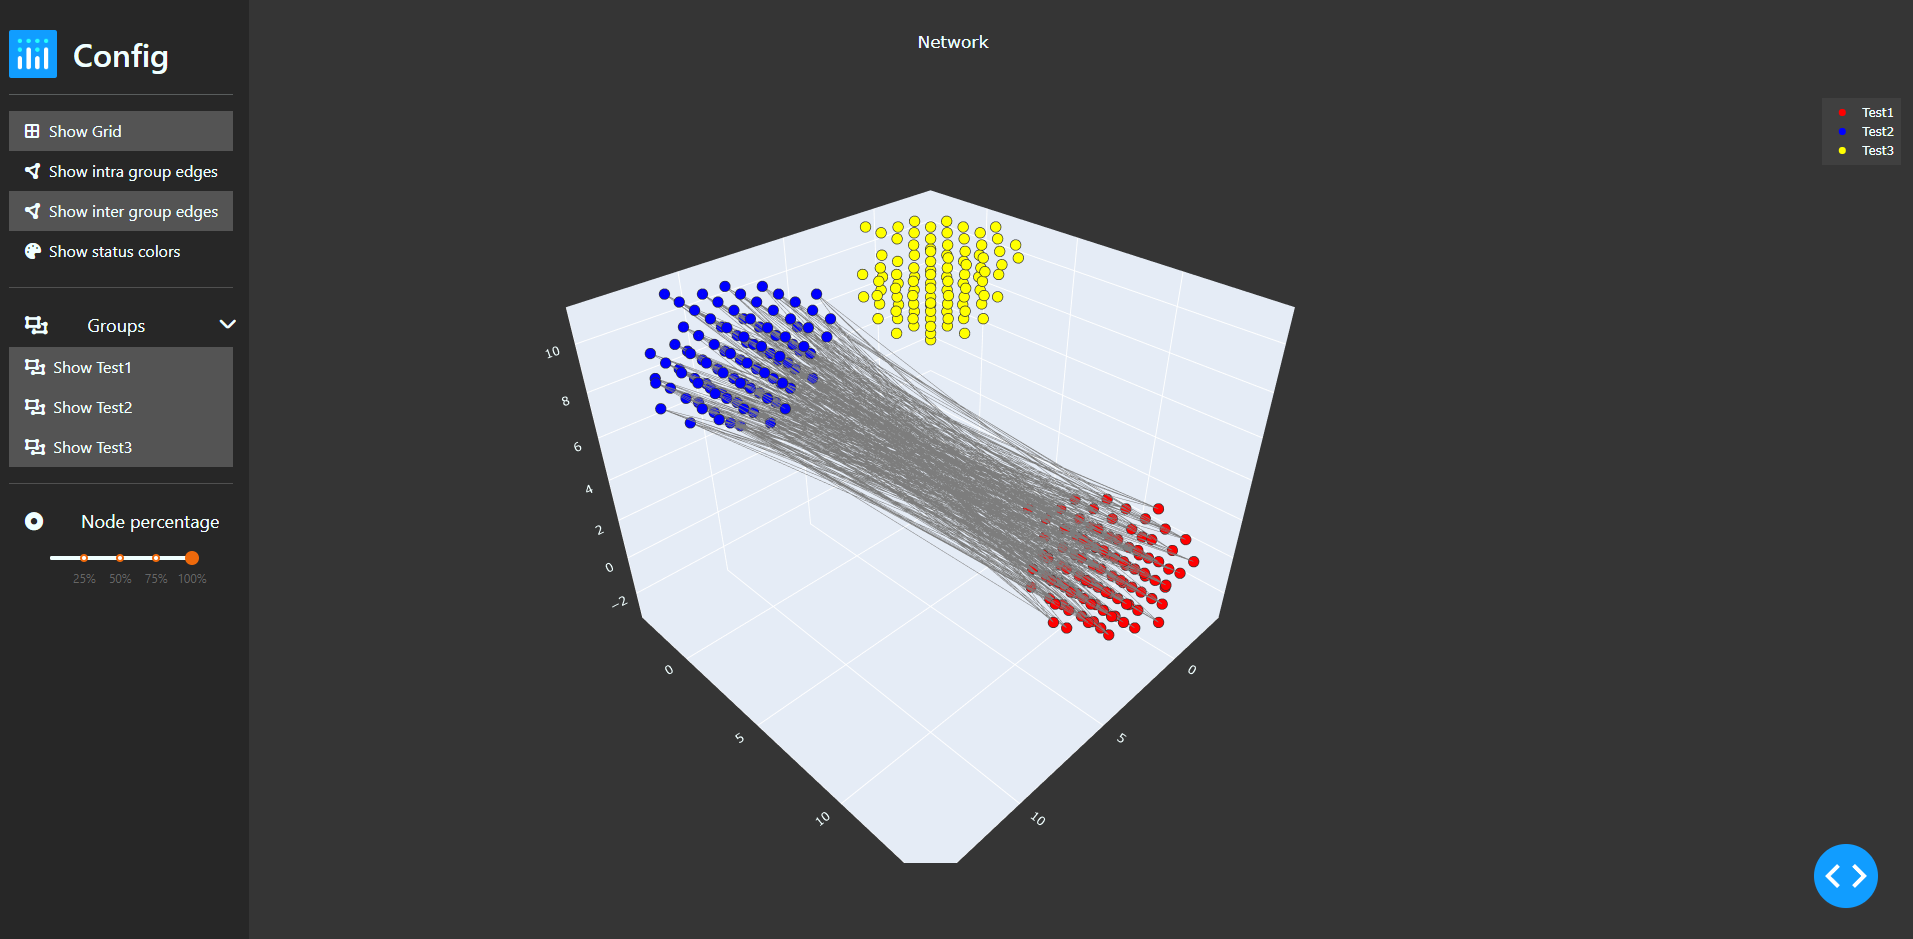
\includegraphics[width=0.5\linewidth]{images/web_network_view.png}
    \caption{UI for the network view webpage}
    \label{fig:web_network_view}
\end{figure}

The sidebar contains buttons to visually disable or enable the grid, intra/inter group edges, group/status color or 
groups of nodes. The slider can be used to reduce the amount of displayed nodes which 
can help to improve performance for large networks. Each of these settings uses a callback
to update the network. Listing \ref{lst:grid_callback} contains one such callback for toggling the grid. This
callback updates the style of the button to change the background color, depending on
whether the button is now activated or deactivated. The \texttt{update\_graph\_grid} edits
the required settings in the plotly figure to enable or disable the grid and then returns
the udpated figure. The two return values of the \texttt{toggle\_grid} function are passed
to the specified outputs which contain the ids of the UI elements for the button and network
figure. By using these outputs dash ensures the changes are represented on the website without
needing to reload it. Similar callbacks are created for the other buttons and the slider.

\begin{lstlisting}[language=python, caption={Callback for toggling the grid}, label={lst:grid_callback}]
@callback(
    [
        Output(self.id_factory("grid-button"), "style"),
        Output(self.id_factory("live-graph"), "figure", allow_duplicate=True),
    ],
    [Input(self.id_factory("grid-button"), "n_clicks")],
    prevent_initial_call=True,
)
def toggle_grid(_):
    self.sidebar.show_grid = not self.sidebar.show_grid
    return {
        "background-color": self.ENABLED_COLOR
        if self.sidebar.show_grid
        else self.BACKGROUND_COLOR
    }, self.update_graph_grid(self.sidebar.show_grid)
\end{lstlisting}

The plotly figure for the network which makes up the rest of the webpage offers some controls
to view the 3D network. The camera can be rotated by holding down the left mosue button
or moved by holding down the right mouse button. The zoom can be changed with the mouse wheel
and in the top right corner there are buttons for these controls as wells as a button to download
the current view as a png. Chapter \ref{cha:network_display} explains how the network figure
is created.

\section{Simulation view}
The simulation view contains the same UI as the network view. Its class inherits from the
network view. Then 5 new buttons to control the simulation are added: reset simulation,
show log outputs, advance one step, turn on auto advancing (1 step per second) and 
save stats. Using these five buttons as wells as the sidebar to control the appearance
of the network, the simulation can be run which will update the graph with new colors
for the current state of each node after each step. This is done in the callback of the
advance step button as shown in listing \ref{lst:step_callback} which runs one simulation
step and then creates the new color sequence and log output. The updated graph and log console
text are then returned to outputs to update the website.

\begin{lstlisting}[language=python, caption={Callback for advancing simulaton by one step}, label={lst:step_callback}]
@callback(
    Output(self.id_factory("live-graph"), "figure", allow_duplicate=True),
    Output("log-console-content", "children", allow_duplicate=True),
    Input(self.id_factory("step"), "n_clicks"),
    prevent_initial_call=True,
)
def step(_):
    with self.sim_mutex:
        self.sim.simulate_step()
        color_map, _ = self.sim.create_color_seq()
        if self.show_logs:
            return (
                self.graph.update_status_colors(color_map),
                self.sim.stats.get_log_text_html(),
            )
        else:
            return self.graph.update_status_colors(color_map), ""
\end{lstlisting}

The reset buttons opens a popup which requires confirmation of the user before the simulation
is actually reset. The save button also opens a popup which allows the user to enter a name
for the statistics of this simulation.

\section{Stats view}
The stats website displays statistics saved during simulations. When the website is first
opened a popup is shown where the user needs to select which statistics to display. This
website contains a similar sidebar as the previous view and simulation sites. The sidebar
contains buttons to control graphs of which statistics are displayed. The UI is depicted in figure
\ref{fig:web_stats_view}.

\begin{figure}
    \centering
    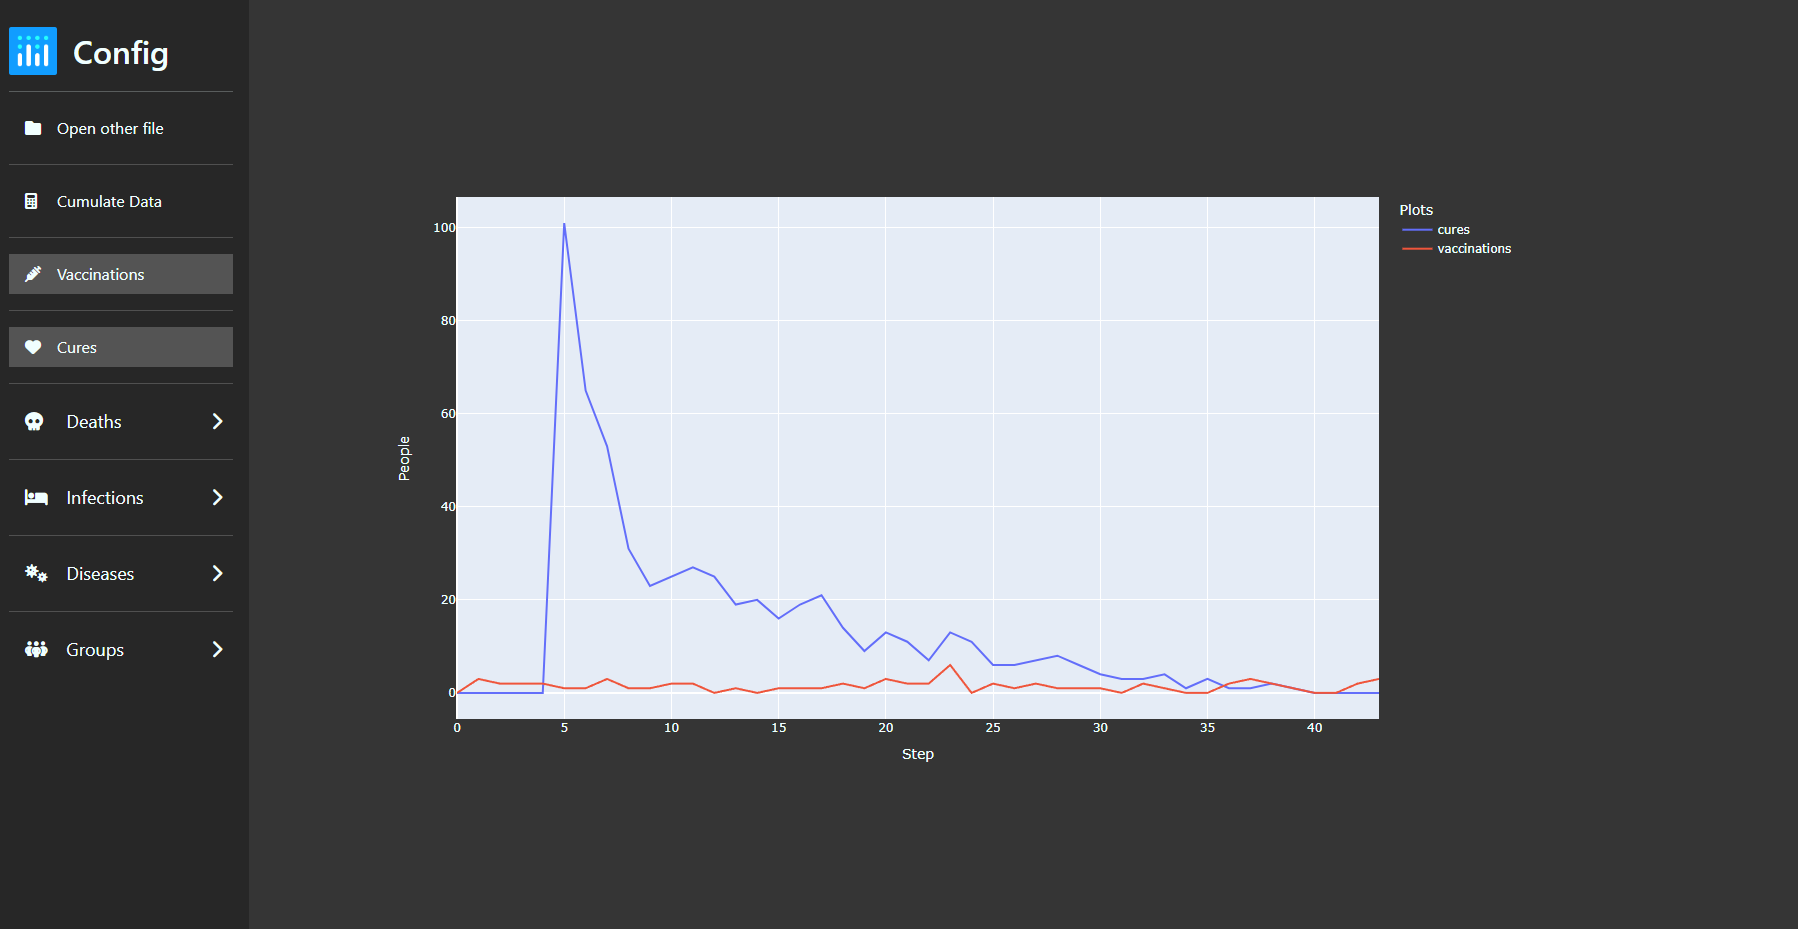
\includegraphics[width=0.5\linewidth]{images/web_stats_view.png}
    \caption{UI for the stats webpage}
    \label{fig:web_stats_view}
\end{figure}

The sidebar contains the following buttons:
\begin{itemize}
    \item Open another file: Brings the popup to select another stat file back up
    \item Cumulate data: Cumulates the graphs to show total up until each step instead of individual values of each step
    \item Display vaccinations, cures, deaths or infections data. Deaths and infections are split
    into total, vaccinated and unvaccinated
    \item Groups and diseases buttons allow to split the data to show only the values for a specific group/disease
    or the total for all diseases/groups
\end{itemize}
These buttons use callbacks to update the graphs similar to the ones for the network view.

\section{Updating the data}
To update the network or availabe stats files that are displayed endpoints are created.
The dash server allows the creation of listeners on URLs which are called if other
applications send HTML POST requests to those URLs. To update the data two endpoints
are exposed, one for updatig the network and one for updating the stat files.
The creation of these endpoints is shown in listing \ref{lst:data_endpoints}.
After a POST request is received the json data it contains is decoded and saved
for the stats or decoded, built and saved for networks. Then the view is reset to update
all open websites. At the end either a response for success (200) or failure (400) is sent.

\begin{lstlisting}[language=python, caption={Endpoints for updating data}, label={lst:data_endpoints}]
@app.server.route("/update-data", methods=["POST"])
def update():
    try:
        json_data = request.get_json()
        project.network = Network.from_dict(json_data)
        project.network.build()
        graph.update_network(project.network)
        html_view.reset()
        sim_view.reset()
        stats_view.reset()
        return make_response(jsonify({"status": "OK"}), 200)
    except Exception as e:
        return make_response(jsonify({"status": {str(e)}}), 400)

@app.server.route("/update-stats", methods=["POST"])
def update_stats():
    try:
        json_data = request.get_json()
        stats = SimStats.from_dict(json_data["stats"])
        project.stats[json_data["filename"]] = stats
        stats_view.reset()
        return make_response(jsonify({"status": "OK"}), 200)
    except Exception as e:
        return make_response(jsonify({"status": {str(e)}}), 400)
\end{lstlisting}


\chapter{Qt}
\label{cha:qt}
Qt is a framework that streamlines the development of high-performance, visually appealing and feature-rich GUI applications. It offers support for multiple languages such as C++, Python, and JavaScript, allowing developers to choose their preferred language. Thanks to the documentation and the large user base, there is a lot of support material to reference \cite{qt}.

With the \hyperref[sub:qt_designer]{Qt Designer}, developers can create GUI designs effortlessly. Designs can be created via drag-and-drop, which accelerates designing in Qt. It also enables developers to visualize what their application will look like in real-time \cite{qt}.

The feature-rich and vast knowledge base, coupled with its user-friendly design, made it an easy choice to use in this project to develop the applications.


\section{Qt Designer}
\label{sub:qt_designer}

This is a tool from the Qt framework that allows designing and building a GUI via drag-and-drop. It uses the what-you-see-is-what-you-get approach, where how it looks in the designer will be the same in the real application \cite{qt}.

Figure \ref{fig:qt_designer} shows the Qt Designer application, which consists of a main window to which widgets can be dragged from the left sidebar to place them in the application. If a layout is selected for the widgets, Qt will automatically fit them according to the layout, so ensuring that the widgets are properly aligned. In applications, it is important to know the hierarchy of the widgets. Qt Designer makes this process easy to figure out, the object window (on the top right) shows the hierarchy tree of the widgets. Making a widget a child of another widget can be achieved by dragging it into the parent widget. 

Not only can the content and placement of the widgets be adjusted, but it is also possible to set several properties of these widgets within Qt Designer (on the bottom right). This helps to see the changes immediately without having to start the GUI application. This is especially useful when changing the style or the layout of certain widgets, as these changes are immediately reflected in the designer.

Qt Designer makes Qt an attractive choice for developers looking to create a GUI application. The real-time visualization makes creating a GUI easy and efficient, making it possible to try out different looks of the application, resulting in a modern-looking design with minimal effort.

\begin{figure}
    \centering
    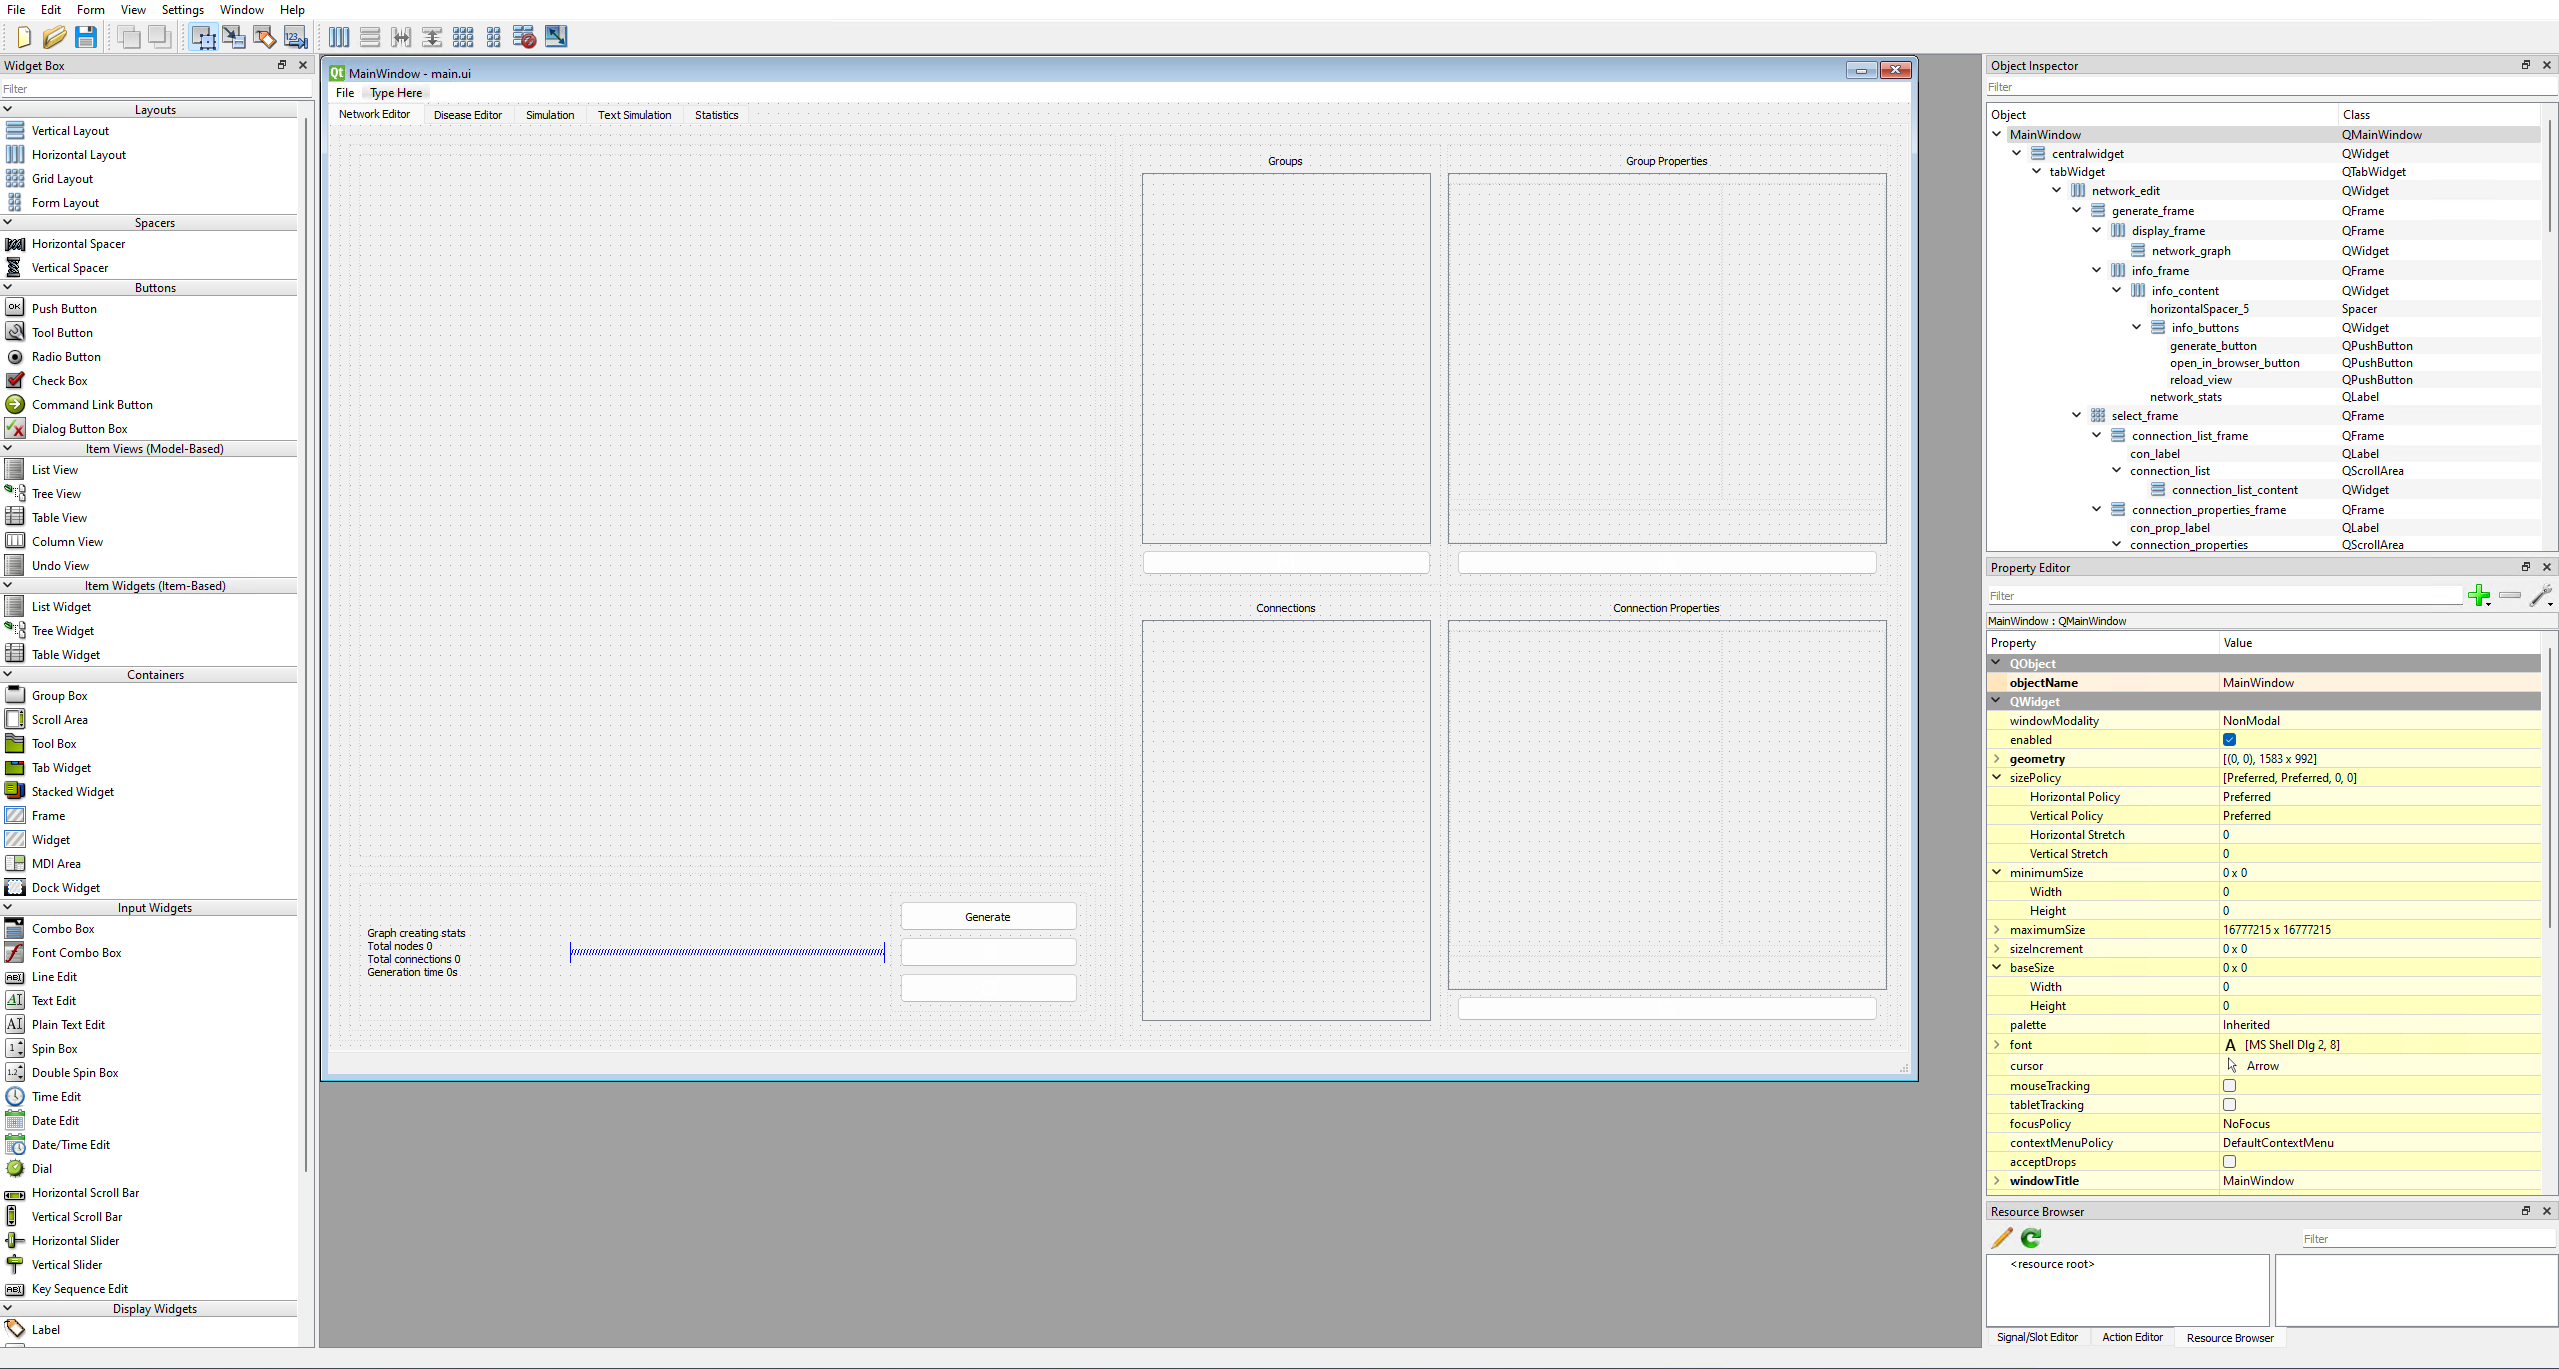
\includegraphics[width=0.8\linewidth]{images/qt_designer.png}
    \caption{Qt Designer}
    \label{fig:qt_designer}
\end{figure}

\section{PyQt}
\label{sub:pyqt}


Qt supports multiple programming languages to allow developers to choose their preferred language. This project was developed in Python, so PyQt was used. PyQt is a module that can be easily installed into the Python environment using pip. It contains all the add-ons that the C++ version of Qt also has. The add-ons can be used by importing the corresponding Python module. 

To develop an application in PyQt, the GUI can either be created using only the Python commands or with the help of the Qt Designer. The GUI created in the Qt Designer is saved in a \textit{.ui} file that can be loaded in the PyQt application \cite{pyqt}. Listing \ref{lst:pyqt_gui} shows how to load a \texttt{.ui} file into a simple application. 

Once a design is loaded into the application, it is easy to access the widgets that were created in the Qt Designer. To access and modify widgets created in the Qt Designer, they can be referenced using the ID associated with the widget in the designer. In Listing \ref{lst:pyqt_gui}, the widget created in the Qt Designer has the ID \textit{myLabel}. Depending on the type of widget, different functions are available, in this case the widget is a label, which contains the \textit{setText} function to change the text it displays. Other widgets, such as a frame widget, offer different functions. 

After a design is loaded, it is possible to add more widgets to it. For example, if buttons need to be created dynamically. This allows developers to create the default design of their application in the Qt Designer and dynamically change the content or arrangement of the widgets in the application. The ease of access to the objects created by the Qt Designer helps to improve the readability and simplicity of the application code.

\begin{lstlisting}[language=python, caption={Simple Qt GUI application}, label={lst:pyqt_gui}]
from PyQt5 import QtWidgets, uic
import sys
class GuiApplication(QtWidgets.QMainWindow):
    def __init__(self):
        super(GuiApplication, self).__init__()
        uic.loadUi('basic.ui', self)
        self.myLabel.setText('Changed text')
        self.show()

app = QtWidgets.QApplication(sys.argv)
window = GuiApplication()
app.exec_()
\end{lstlisting}

\section{Signals and Slots}
\label{sub:signals}

In GUI programming, it is often necessary to execute functions when, for example, a button is pressed. Other frameworks use callbacks to achieve this functionality; Qt uses the signals and slots mechanism. The signal is emitted by an object when its internal state changes. The slot is the function that will be executed once the corresponding signal is emitted. A signal can have multiple slots connected to it, which are executed one after the other. The signal-slot mechanism is independent of the GUI event loop and is executed immediately after a signal is emitted \cite{qt}.

Each signal has a \textit{.connect(Slot slot)} function that is used to connect the signal to a slot. For example, a button in Qt has three signals: \textit{clicked}, \textit{pressed}, and \textit{released}. In order to connect a function to the button, the following command has to be used: \textit{example\_button.clicked.connect(slot\_function)}. Now, when the button is clicked by the user in the GUI, the \textit{slot\_function} is executed \cite{pyqt}.

In this project, the signals and slots feature is mainly used to connect button presses and allow different objects to communicate with each other. The reason why signals should be used for objects to communicate with each other is explained in section \ref{sub:thread_communication}. Listing \ref{lst:signal_slot_example} contains a simple example from the project, that allows the user to start the network generation with a button press. To be able to start the generation process, the \textit{clicked} signal of the button \textit{generate\_button} is connected to the method \textit{start\_generating}. When the user presses the button, the slot is executed and therefore the generation process is started.
\begin{lstlisting}[language=python, caption={Signals and Slots example from the project.}, label={lst:signal_slot_example}]
class UiDisplayGroup(QObject):
    ...
    def connect_signals(self):
        self.generate_button.clicked.connect(self.start_generating)
        ...
    def start_generating(self):
        # Start the thread to generate the network.
\end{lstlisting}

\subsection{Thread communication}
\label{sub:thread_communication}

In general, it is bad practice to have a thread modify GUI widgets to ensure separation of concerns. If this thread were killed prematurely, it could result in an unexpected GUI state that could lead to errors. Or, if the main thread changed the structure of the GUI widgets before the thread could add the desired widgets, this would also lead to errors. To solve this issue, the signals and slots mechanism is ideal for this situation. Instead of letting a thread handle the widget creation, the thread just sends the widget data back to the main thread, which then adds or modifies the widgets. This way, the integrity of the GUI can be maintained because the main thread retains control over widget manipulation, ensuring consistent and expected behavior \cite{qt}.

An example of this approach is shown in listing \ref{lst:pyqt_thread_comm}. It demonstrates how the text simulation updates the label showing the current simulation speed. To achieve this functionality, three different classes were used:
\begin{description}
    \item[UiTextSimulationTab:] This runs in the main thread and changes the widgets.
    \item[SimulationWorker:] This class executes the simulation in a separate thread.
    \item[WorkerSignals:] This class only holds the signals that the threads can send.
\end{description}
First, an object for the class \textit{WorkerSignals} is created and stored as \textit{worker\_signals} in the \textit{UiTextSimulationTab}. The signals of this class are assigned to slots in the \textit{connect\_signals} method. Here, the \textit{update\_control\_label\_signal} is connected to the method \textit{update\_control\_labels}. When a user presses the buttons that changes the simulation speed, a signal is sent that executes the \textit{change\_speed} method that has been connected to the slot. This method changes the simulation speed according to the action sent as parameter. After changing the speed, this method sends the signal \textit{update\_control\_label\_signal}. This signal contains the current simulation speed. The simulation speed sent by the signal is received by \textit{update\_control\_labels}, which is executed in the main thread and can safely update the label containing the information. This way, only the main thread will change widgets.
\begin{lstlisting}[language=python, caption={Thread safety example}, label={lst:pyqt_thread_comm}]
class WorkerSignals(QObject):
    update_control_label_signal: pyqtSignal = pyqtSignal(float)
    ...
class SimulationWorker(QThread):
    ...
    def change_speed(self, action: str):
        # Changes the simulation speed according to the received action.
        self.signals.update_control_label_signal.emit(self.simulation_speed)
class UiTextSimulationTab:
    def __init__(self, parent: QtWidgets.QMainWindow):
        ... 
        self.worker_signals = WorkerSignals()
        ...
    def connect_signals(self):
        # Connecting the button Signals and other signals from the worker_signals
        self.worker_signals.update_control_label_signal.connect(self.update_control_labels)
    def update_control_labels(self, simulation_speed: float):
        # Updating the labels containing the simulation speed information.
\end{lstlisting}

\section{QSS}

Like HTML, Qt supports a style sheet to specify how widgets should look. QSS was inspired by CSS (Cascading Style Sheets) and is therefore very similar in terminology and syntax. A style sheet can be set for each widget either directly in the Qt Designer, in the code or in a separate file. If widgets are created dynamically and are not present in the Qt Designer, it is not possible for the Qt Designer to set the style for these widgets. In this case, either a style sheet file is needed, or the style must be set in the program itself \cite{qt}. The style sheet file has the advantage that it contains all the styles in one place rather than scattered throughout the program, which improves maintainability. The syntax for a style sheet is shown in listing \ref{lst:qss_example}. In this example, the padding and spacing for the \textit{QCheckBox} are changed. When a \textit{QCheckBox} is checked, it will display an image with the specified width and height.
\begin{lstlisting}[language=python, caption={QSS example}, label={lst:qss_example}]
QCheckBox{
    padding: 0px;
    spacing: 0px;
}
QCheckBox::indicator:checked {
    image: url(assets:selected.png);
    width: 24px;
    height: 24px;
}
\end{lstlisting}

To load a style sheet, it must first be loaded and then set as the style in the main application. PyQt5 has a method \textit{setStyleSheet} for every widget in Qt, which can be used to set individual styles for different widgets. It is also possible to set the style for the main application, which is used by all widgets in that application but is overridden by individual widget styles. Listing \ref{lst:load_qss}, shows how to set the style sheet as the main window style after successfully reading it \cite{pyqt}.
\begin{lstlisting}[language=python, caption={Loading of the QSS}, label={lst:load_qss}]
class UiNetworkEditor(QtWidgets.QMainWindow):
    ...
    def load_window(self):
        ...
        with open("qt/NetworkEdit/style_sheet.qss", mode="r", encoding="utf-8") as fp:
            self.stylesheet = fp.read()
        self.setStyleSheet(self.stylesheet)
\end{lstlisting}



\section{Abblication views}
\label{sub:thread_views}
The GUI application of the created app, contains five tabs/views, each with a different use:
\begin{description}
    \item[Network Editor] In this view, the user can create a network consisting of nodes and connections and view it in a 3D space.
    \item[Disease Editor] Allows to create the disease that are used for the simulation in the created network.
    \item[Simulation] The Simulation view embeds the webpage used for simulation. It displays the network and its state during the simulation, allowing the user to observe the behavior of the disease in the network.
    \item[Text Simulation] If the network is too big or a large number of simulation cycles are required, which makes using the visual simulation impractical, this text-based simulation can be used instead. It provides the same functionality for controlling the simulation and saving statistics as the visual simulation.
    \item[Statistics] This view embeds the webpage used to display the saved statistics. It can be used to view graphs for the various stats saved during simulations to help analyze the results.
\end{description}

\chapter{Experiments}
\label{cha:experiments}
In this chapter some experiments will be conducted. These experiments are modeled
after the scenarios described in the Theory chapter %TODO ref
The goal is to recreate these situation using the developed tool and running a
simulation with the described parameters. These simulations can then be used
to support or refute the assumptions that were made on how the diseases
theoretically should behave in those scenarios.

\section{Importance of $R_0$}
The role of the reproductive number $R_0$ was discussed in section \ref{sub:r0}.
It is the deciding factor for whether a disease is dying out ($R_0 < 1$) 
or able to live indefinitely ($R_0 > 1$). Calculating $R_0$ in complex social
networks is very hard because the structure of the networks has a big impact on $R_0$
in addition to the characteristics of the disease. For these experiments a very
rough estimation of $R_0=e_\mu \cdot p$ is used as this is sufficient for estimating whether
the disease should die out in the experiment or life for a long time.
$e_\mu$ is the average amount of connection per node, let $N$ be the total
amount of nodes in the network and $E$ the total amount of edges then
$e_\mu=\frac{E}{N}$. $p$ is the probability for a node to get infected
if one of its neighbors has the disease.

\subsection{The network}
\label{sub:exp_network}
The network that is used in these experiments contains 3 groups with 5000 nodes
each. Group 1 has 5 intra group connections for each node, group 2 has 4 and
group 3 has 3 intra group connections. Between each pair of groups there are
2 connections per node. The resulting network can be seen in figure %TODO
It contains a total of 15,000 nodes. Let $N_i$ be the amount of nodes in group $i$
then the amount of edges can be calculated using the following equation:
\begin{equation}
    E = \frac{n_1}{2} * 5 + \frac{n_2}{2} * 4 + \frac{n_3}{2} * 3 + \frac{n_1+n_2}{2} * 2 + \frac{n_1+n_3}{2} * 2 + \frac{n_2+n_3}{2} * 2
\end{equation}
Using that equation the it can be calculated that the network contains 60,000 edges.
This leads to an average amount of connections per node of $e\mu=\frac{60,000}{15,000} = 4$.

\subsection{Experiment with $R_0 < 1$}
Since this experiment will use the same network as the one for a $R_0 > 1$ the
facor $e_\mu$ is static and cannot be changed. This makes $p$ the only deciding
factor for $R_0$ it can be calculated using $p = \frac{R_0}{e_\mu}$ so in this case
with $R_0 < 1$, $p < \frac{1}{4}$. For cases with $R_0$ close to 1 there is still
a decent chance that the disease will live for a long time which is why $p=0.125$
is chosen for a estimated $R_0=0.5$ to ensure that the disease dies out in a finite
amount of steps.

The parameters for the disease of this experiment then are:
\begin{itemize}
    \item %TODO
\end{itemize}

Running the simulation shows that the disease is never able to spread to a large
amount of people and dies out after only \~ %TODO
steps. This can also be seen in the graph %TODO 
which shows the amount of new infections per cycle. 
Increasing the initial amount of infected nodes to 5,000 shows that even with
such a large amount of infections the disease dies out after a certain amount of steps.
In this case it took %TODO
steps, graph %TODO
shows the amount of new infections up to that point.

This experiment supports the theory that for a $R_0 < 1$ the disease will die out
in a finite amount of steps.

\subsection{Experiment with $R_0 > 1$}
This network uses the same network as the previous one, so $p$ is again the deciding
factor for $R_0$. $p = \frac{R_0}{e_\mu}$ so for this case with $R_0 > 1$, $p > \frac{1}{4}$
since the closer $R_0$ to 1 the higher the chance the disease dies out $p=0.375$ is chosen
resulting in a $R_0 = 1.5$.

The properties that were changed from the previous experiment are:
\begin{itemize}
    \item %TODO
\end{itemize}

After running the simulation for 2,000 cycles the disease is still alive and infecting
new nodes. This supports the theory that with a $R_0 > 1$ there is a probability $> 0$
that the disease never dies out. Figure %TODO
shows the amount of new infections which is remains relatively constant 
from cycle x to %TODO.

\subsubsection{Changing the network}
To show that the network structure indeed has an impact on $R_0$ this experiment
uses the same disease as the previous one. The network will have only half as many
edges, group 1 has 2 intra group connections for each node, group 2 has 2 and
group 3 has 2 intra group connections. Between each pair of groups there are
1 connections per node. This new network has 30,000 edges resulting in $e_\mu$ = 2.
Thus the new estimated $R_0=2\cdot0.375=0.75$ which is smaller than 1 so they
expectation is that the disease will die out even though it has the same infection 
rate as before.

After %TODO
cycles the disease has died out which supports the theory that the network structure
has an impact on the spreading of diseases along with the characteristics of the disease.
Graph %TODO 
shows the amount of infections until the disease died out.

\section{Multiple Diseases}
Interesting dynamics can be observed if multiple diseases are introduced into the same
social network. Cases with two diseases where one or both of the diseases have a $R_0 < 1$
do not make for an interesting scenario as once one disease has died out the problem just
gets reduced to one disease. But if both (or more) diseases have a $R_0 > 1$ then they 
will compete against each for survival, assuming a person can only be infected by one diseases
at a time, for example because they stay at home until they are cured so they can not get
infected by another disease during that period. Since a disease needs to constantly infect
new nodes to stay alive the diseases can rot other diseases out by infecting all nodes themselfes
thus leaving no availabe nodes to infect for other diseases.

For diseases with a similar $R_0$ the two diseases will each have \~50\% of infections.
Now consider a case where one diseases $d_1$ has $R_0^1=2$ and the second $d_2$ has $R_0^2=5$.
When the diseases are viewed in isolation theoretically both are able to survive as both
$R_0^1 > 1, R_0^2>1$. Looking at the situation where both diseases are in the same network,
$d_2$ will infect significantly more people than $d_1$, about 2.5 times as many. This means
that $d_2$ will have $~\frac{5}{7}$ of total infections during the first wave. As $d_2$ has
way more infected nodes during the first wave that makes it even easier for it to spread than
$d_1$. At the borders where susceptible nodes have connections to nodes infected with $d_1$
and also to nodes infected with $d_2$, $d_2$ will infect $\frac{5}{7}$ of those nodes. This
will slowly reduce the amount of nodes infected with $d_1$ until none are left and $d_1$ has died
out even though its $R_0^1>1$. This means in networks with more than one disease the one 
with the highest $R_0$ value is the one most likely to survive.

\subsection{Experiment}
This theory can again be supported by conducting an experiment using the developed simulation
tool. The network will be the same used in the previous experiment, consisting of 3 groups with
more intra group connections than inter group connections. The exact structure is explained
in section \ref{sub:exp_network}.

Two diseases are used for this simulation:
\begin{itemize}
    \item %TODO
\end{itemize}

First the experiment is run with the two diseases separately to show that they never die out
on their own. The results can be seen in figure %TODO
which shows the amount of new infections until cycle %TODO
indicating that the diseases have not died out until then.

Now both diseseases are used at the same time. After only %TODO cycles
$d_1$ has died out because the new infections of $d_2$ have increased so much that
no new nodes are availabe for $d_1$ to infect. This increases in infections with $d_2$ and
decrease in infections with $d_1$ is shown in figure %TODO

This supports the theory that in networks with multiple highly infectious diseases the
one with the highest $R_0$ value is the one most likely to survive.

\section{Small-World Phenomenon}
The small-world phenomenon is also known as six degrees of separation. The theory is that
in an arbitratily large social network the length of the path from one person to any other
person is on average only 6 steps long. To support this theory Stanley Milgram conducted
an experiment in the 1960s \cite{smallWorld}. In this experiment Milgram gave a letter to 
a random source person in Nebraska (US) and told them to deliver it to a target person in
Massachusetts (US). The source person was only given basic information about the target like 
address and occupation and each person was only allowed to send the letter to someone they
knew on a first name basis with the goal to get the letter closer to its target. Any person
in this chain was given the same information. After many iteration of this experiment the 
average amount of persons it took to deliver the letter to its target was between 5 and 6 persons
leading to the name of the six degrees of separation principle.

This experiment does not always find the shortest path though as the people forward the letter
only to the person they assume to be closest to the target. Unkownst to them there might
be another person they know who is much closer to the target making for a shorter path which
is never discovered. To find the true shortest path each participant would have to forward
the letter to all their friends while keeping track of which path the letter has taken.
Then after all letters have arrived at the target the true shortest path is the one of the
letter that needed the least amount of persons to arrive.

\subsection{Experiment}
For this experiment a network with only one group is created. That group
contains 10,000 nodes with each node having %TODO
connections. Though this network is not totally accurate to a real situation. Usually 
a friends network of a person is tightly coupled, the friends of a person usually also know
each other and their friends know the initial person etc. Also a person mostly knows
others that live in an area close to them and only fewer persons that live farther away.
This leads to a highly connected network with only short connections and a few random longer connections.
The network used for this experiment uses only random edges which does not represent this
fact that the geolocically closer people are the more connections they have. However in the
current day the internet allows for way more connections over long distances which makes
the used network more valid in that context.

\begin{figure}
    \centering
    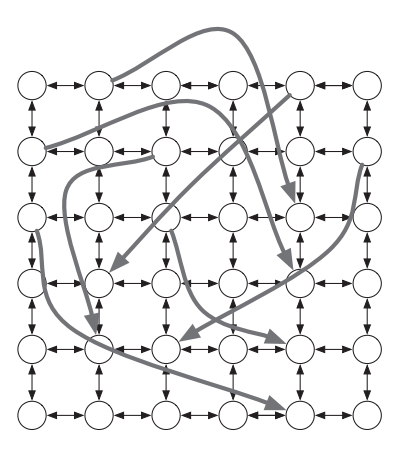
\includegraphics[width=0.5\linewidth]{images/sw_true_network.png}
    \caption{True structure of a network showing the friends of persons. The
    geolocically closer people are the higher the amount of connections. There
    are only few connections over longer range. (source: \cite{networks})}
    \label{fig:oscillation}
\end{figure}


To show that each node can be reached in only six steps, a disease with an infection rate
of 1 and infection duration of 1000 is used. Initially only one
node is infected. Figure %TODO shows the network after x cycles.
After cycle %TODO
all nodes are infected which means they were all able to be reached from the 
starting node in only %TODO
steps.

To reduce the limitation of the used network in regards to the random connections another
network structure could be used. This one closer models the existance of highly coupled
local friend groups where everyone knows each other and a few random connections to people
from other friend groups who are further away. This network uses a high amount of
groups with relatively few members each. In this case 100 groups of 5-10 people are used
and each group of people is connected to 3-4 other groups with only 2-3 edges each.

The same disease is used in this network and the state of the network after cycle %TODO
can be seen in figure %TODO
This shows that in this network it is also possible to reach all other nodes in only six steps,
even though there are only a few long distance connections and a lot of thightly coupled
small groups.




\chapter{Summary and Outlook}
\label{cha:summary}
\section{Achieved Results}
In chapter \ref{cha:general_principles} the theory of epidemics was introduced. The two main parts of epidemics were discussed, networks and diseases. Three existing models and their respective limitations were explained, a simple tree-based model, the SIR Model and the SIS Model. These were  combined and extended to create the custom model used in this work. This custom model was explained in detail in section \ref{sec:custom_model}.

An app was created that uses the custom model to allow for simulations of epidemics. The app includes functions for modeling social networks, creating diseases, running simulations with the created networks and diseases and collecting statistics about the simulation. The general functionality of the app has been outlined in chapter \ref{cha:implementation} and its implementation is described in chapters \ref{cha:network_generation}, \ref{cha:network_display} and \ref{cha:visual_simulation}, which explain the process and algorithms involved in creating the app.

After creating the app some experiments were conducted to support the theories discussed in chapter \ref{cha:general_principles}. These experiments were performed using the developed app. The results of the simulations coincided with the theories of how the diseases are expected to behave. This indicated the importance of factors like the reproductive number $R_0$ in epidemics. The findings of these experiments and theories can be used to better prepare for real-world scenarios of epidemics. They help to understand the behavior of diseases and their lifetime in complex social networks.

\section{Outlook}
\subsection{Extensibility of the Results}
The network editor can be extended to allow precise control over which nodes are connected to which. This requires a solution that still allows fast creation of large networks while providing such fine control over the connections.

For very large networks, the computation can take a long time. Tests showed that networks with \~100,000 nodes took almost 30 minutes to generate. A big factor for this long time is that Python is an interpreted language, which makes such calculations relatively slow compared to the same calculations in a compiled language like C++. The app could be reimplemented in C++ which would reduce the computing time, but since C++ does not provide a package like plotly, a custom implementation for displaying the graphs is necessary, which can be time consuming to implement.

\subsection{Transferability of the Results}
The results achieved using the simulation can be applied to real-world scenarios. These simulations can help to predict how an epidemic will evolve over time. This can be used to test how certain factors affect the spreading of the disease to determine what countermeasures are necessary to suppress the disease and ensure the safety of the population. One example might be reducing the number of connections in the network, which could be achieved in the real world by implementing social distancing measures. Another factor that can be tested is whether a vaccine that reduces the infection probability by a certain amount is sufficient to make the disease die out or what percentage of people would need to be vaccinated to achieve this.

Without tools to simulate the behavior of diseases, it is almost impossible to predict what will happen, making it difficult to decide on the necessary countermeasure until it might be too late. This is why tools for simulation are necessary in the field of epidemics.


% \chapter{Introduction}
% \label{cha:introduction}
% \section{Motivation}
An epidemic outbreak can have a major impact on the world. Past epidemics have shown that
if we do not know how to counteract an epidemic outbreak and are not prepared for 
such cases, a new disease can cause the death of major parts of the world. The black
death caused the death of about 30\% to 60\% of all Europeans (75-200 million)
during the 1300s \cite{blackDeath}.
To better understand such scenarios simulations play an important role since studying real
cases of epidemic outbreaks is difficult as there are only so many in the history of humans.
Also it is important in case an outbreak happens to be able to simulate the next few days/weeks
to accurately predict how the epidemic will evolve.

For this reason this work will discuss an approach to simulate such epidemics by modeling
networks of persons and then simulating the spreading of diseases with different properties
in these networks.

\section{Problem definition}
A model of the social network the disease is spreading in is curcial to the simulation.
Depending on the transmission method of the disease this network can be highly connected in 
the case of a disease with airborne transmission or have only few connections for diseases
that are for example sexually transmitted. In addition to that different diseases can spread
completely different in the same social network even if the have the same transmission method
because the characteristics of the disease also play an important role in how it spreads. 
As suggested by Easley and Kleinberg \cite{networks}
the transmission of computer viruses works in a similar way an thus is also able to be modeled
by using networks.

The networks that can be created using the app must be able to model different social
networks. The important part for the epidemics simulation is the modeling of the amount
of contacts with other humans each human has. Since each group can contain a significant amount
of members an efficient method for creation networks with large amounts of nodes is required, which
still allows to model most social networks.

A method to visually display these networks in a clear way is required. The visual 
representation must still be usable with large amounts of nodes (eg. over 100,000 nodes).
To make the visualization of the network more usable some settings need to be provided
to alter the displayed network, like hiding certain connections or nodes. It also needs
ways to represent the current state of the network in respect to the spread of the diseases.

The app also needs to allow for creation of multiple diseases with different properties.
To simulate various epidemic scenarios properties like the infectiousness, duration of illnes
or fatality need to be editable. 

The app should be able to simulate multiple diseases at the same time. The simulation needs
to take into account which humans have contact with each other and then simulate the spreading
of the diseases according to the properties of each disease and group of humans.

During the simulation the app will collect statistics to allow a review of key information
after a simulation, like the amount of new infections over time.

% \chapter{Terminology}
% \label{cha:terminology}
% \input{tex/terminology}

% \chapter{Defining different types of Games}
% \label{cha:gameDefinitions}
% \input{tex/gameDefinitions}

% \chapter{Solution Strategies and Nash Equilibria}
% \label{cha:solutionStrategies}
% \input{tex/solutionStrategies}

% \chapter{Complexity of finding Nash equilibria}
% \label{cha:complexityOfFindingNash}
% \input{tex/complexityOfFindingNash}

% \chapter{Summary}
% \label{cha:summary}
% \section{Achieved Results}
In chapter \ref{cha:general_principles} the theory of epidemics was introduced. The two main parts of epidemics were discussed, networks and diseases. Three existing models and their respective limitations were explained, a simple tree-based model, the SIR Model and the SIS Model. These were  combined and extended to create the custom model used in this work. This custom model was explained in detail in section \ref{sec:custom_model}.

An app was created that uses the custom model to allow for simulations of epidemics. The app includes functions for modeling social networks, creating diseases, running simulations with the created networks and diseases and collecting statistics about the simulation. The general functionality of the app has been outlined in chapter \ref{cha:implementation} and its implementation is described in chapters \ref{cha:network_generation}, \ref{cha:network_display} and \ref{cha:visual_simulation}, which explain the process and algorithms involved in creating the app.

After creating the app some experiments were conducted to support the theories discussed in chapter \ref{cha:general_principles}. These experiments were performed using the developed app. The results of the simulations coincided with the theories of how the diseases are expected to behave. This indicated the importance of factors like the reproductive number $R_0$ in epidemics. The findings of these experiments and theories can be used to better prepare for real-world scenarios of epidemics. They help to understand the behavior of diseases and their lifetime in complex social networks.

\section{Outlook}
\subsection{Extensibility of the Results}
The network editor can be extended to allow precise control over which nodes are connected to which. This requires a solution that still allows fast creation of large networks while providing such fine control over the connections.

For very large networks, the computation can take a long time. Tests showed that networks with \~100,000 nodes took almost 30 minutes to generate. A big factor for this long time is that Python is an interpreted language, which makes such calculations relatively slow compared to the same calculations in a compiled language like C++. The app could be reimplemented in C++ which would reduce the computing time, but since C++ does not provide a package like plotly, a custom implementation for displaying the graphs is necessary, which can be time consuming to implement.

\subsection{Transferability of the Results}
The results achieved using the simulation can be applied to real-world scenarios. These simulations can help to predict how an epidemic will evolve over time. This can be used to test how certain factors affect the spreading of the disease to determine what countermeasures are necessary to suppress the disease and ensure the safety of the population. One example might be reducing the number of connections in the network, which could be achieved in the real world by implementing social distancing measures. Another factor that can be tested is whether a vaccine that reduces the infection probability by a certain amount is sufficient to make the disease die out or what percentage of people would need to be vaccinated to achieve this.

Without tools to simulate the behavior of diseases, it is almost impossible to predict what will happen, making it difficult to decide on the necessary countermeasure until it might be too late. This is why tools for simulation are necessary in the field of epidemics.


%-----------------------------------------------------------------------
\appendix

%---
\printbibliography[heading=bibintoc]

\end{document}